\documentclass [11pt, letterpaper] {article}
\input {headings}
\newcommand \recipeName {BBQed Pork Back Ribs}
\newcommand \fileName {BBQedPorkBackRibs}
\chead {\recipeName}

\begin {document}
\input {title}

\begin{flushright}
{From Mario Batali.}
\end{flushright}


During the COVID-19 pandemic we were all isolating at home. We started having virtual dinner parties where we would contact a few friends, each prepared a dinner and got a glass of wine at their own homes, and we sat down in front of a teleconferencing system for a conversation. In one of those Sheri Sommervile said that her son Jason and herself wanted to make a fall-of-the-bone BBQed ribs. Thus, I adapted my \href{BBQedChickenDrumSticks.html}{BBQed Chicken Drumsticks} recipe especially for them.

\begin{description}

\item[Ingredients:]\ \\
	\begin{itemize}
	\item 6 pounds of  pork back rib
	\item 1 Tablespoon of table salt
	\item 1 Tbs cumin seeds
	\item 1 teaspoon whole black peppercorn kernels
	\item 2 Tablespoon chili powder
	\item 1 Tablespoon paprika
        \item 1 teaspoon of dried oregano
	\item Cooking spray
	\item 1 cup of barbecue sause (I use Bull's Eye)
	\item 1/2 cup of ketchup
	\end{itemize}
\item[Equipment and Supplies:]\ \\
	\begin{itemize}
	\item rimmed baking sheet
	\item a small coffee grinder that you use for spice grinding
	\item aluminum foil
	\end{itemize}

\item[Procedure:]\ \\
	\begin{enumerate}
	\item {\bf Remove silver skin from back ribs:}
		\begin{itemize}
		\item Rinse ribs over cold water and pat dry with paper towels.
		\item Place the ribs with the bone side up on a rimmed baking sheet.
		\item Use a sharp pairing knife to lift the edge of the silver skin attached to the bones. 
		\item Use a clean and dry paper towel to grab the skin, hold the ribs with one hand and pull the skin off with the other. The whole skin should come off with one pull. If it does not, use the pairing knife to repeat the process.
		\end{itemize}
	\item {\bf Season the Ribs with Salt and a Dry Rub}
		\begin{itemize}
		\item Sprinkle the salt on both sides of the rib racks.
		\item Put the cumin seeds and the whole black peppercorn kernels in the skillet.
		\item Dry roast these spices for a few minutes until they are very aromatic but not burned.
		\item Dump the roasted spices in a small coffee grinder that you use for spice grinding.
		\item Grind the freshly roasted spices to a powder and dump into a small bowl.
		\item Add the chilli powder and the paprika to the spice bowl and stir well.
                \item Rub the dry oregano on the palm  of your hands to release the oils and mix with the spice mixture.
		\item Remove the air-dried chicken from the rimmed baking sheet and put in a container with cover.
		\item Sprinkle the spice mixture on both sides of the rib rack. 
		\item You can proceed to the slow roasting but it is best if you cover and let it rest in the fridge for at least one hour. You can also refrigerate overnight.
		\end{itemize}
	\item {\bf Slow roast the ribs}
		\begin{itemize}
	        \item Spray aluminum foil with cooking spray.
		\item Cover the rimmed baking sheet with the foil.
		\item Place the baking sheet in the oven and turn the oven to 325F. Slow roast the ribs for 1 1/2 to 2 hours. The meat should be tender and easily come out of the bones when pulled. 
                 \item Do not tear the foil when removing it
		\item The pork will release juices during this baking. Do not throw away the juice.
		\end{itemize}
	\item {\bf Coat with barbecue sauce}
		\begin{itemize}
		 \item Remove the pork from the oven.
		 \item Increase the oven temperature to 400 F.
		 \item Use the same foil placing its clean side down on a clean rimmed baking sheet.  
                 \item Place de ribs on top of the foil.
		\item Mix barbecue sauce with ketchup and about 1/2 cup of the liquid that was released from the first baking of the ribs in a small bowl.
		\item Spread the barbecue sauce mixture ensuring to coat only the ribs.
		\item Return the ribs to the oven for another 10 minutes or so until the sauce has dried a bit but is still shiny.
		\item Let cool for several minutes before serving. 
		\end{itemize}
     	\end{enumerate}         
\end{description}
\begin{table}
\begin{tabular}{cccc}
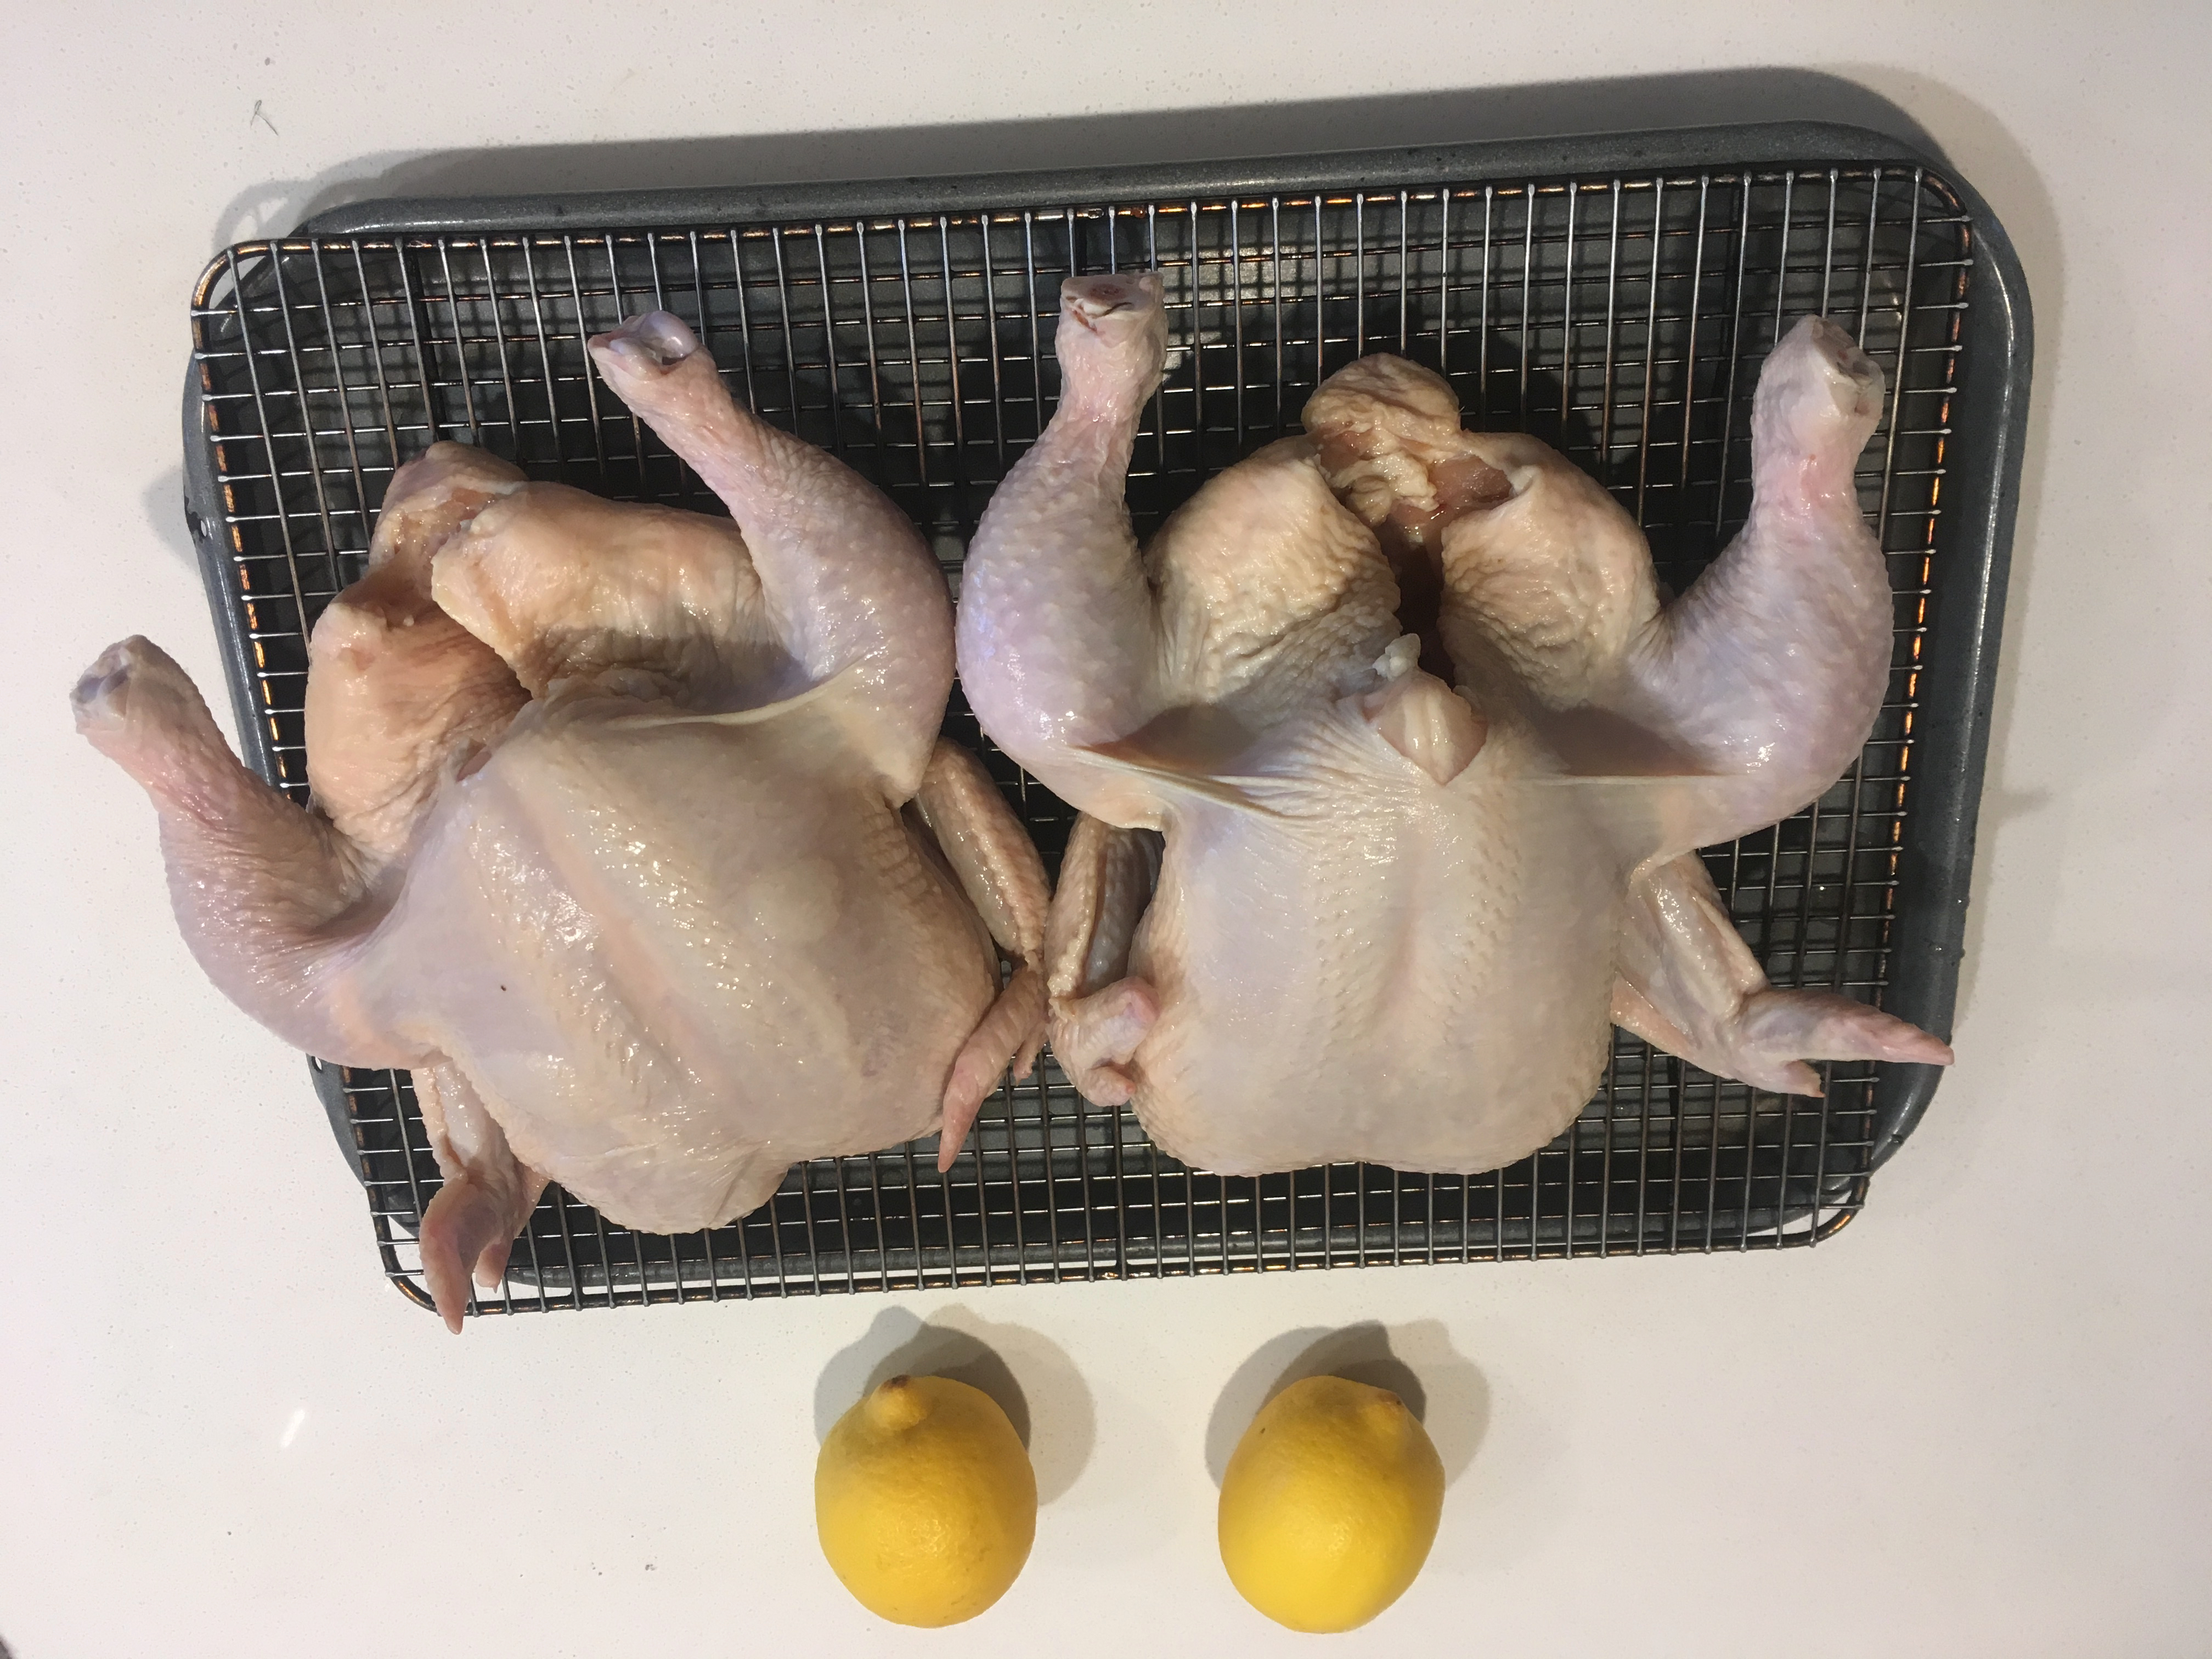
\includegraphics[width=0.25\textwidth]{\imageDir/\fileName/IMG_3197.jpg} &
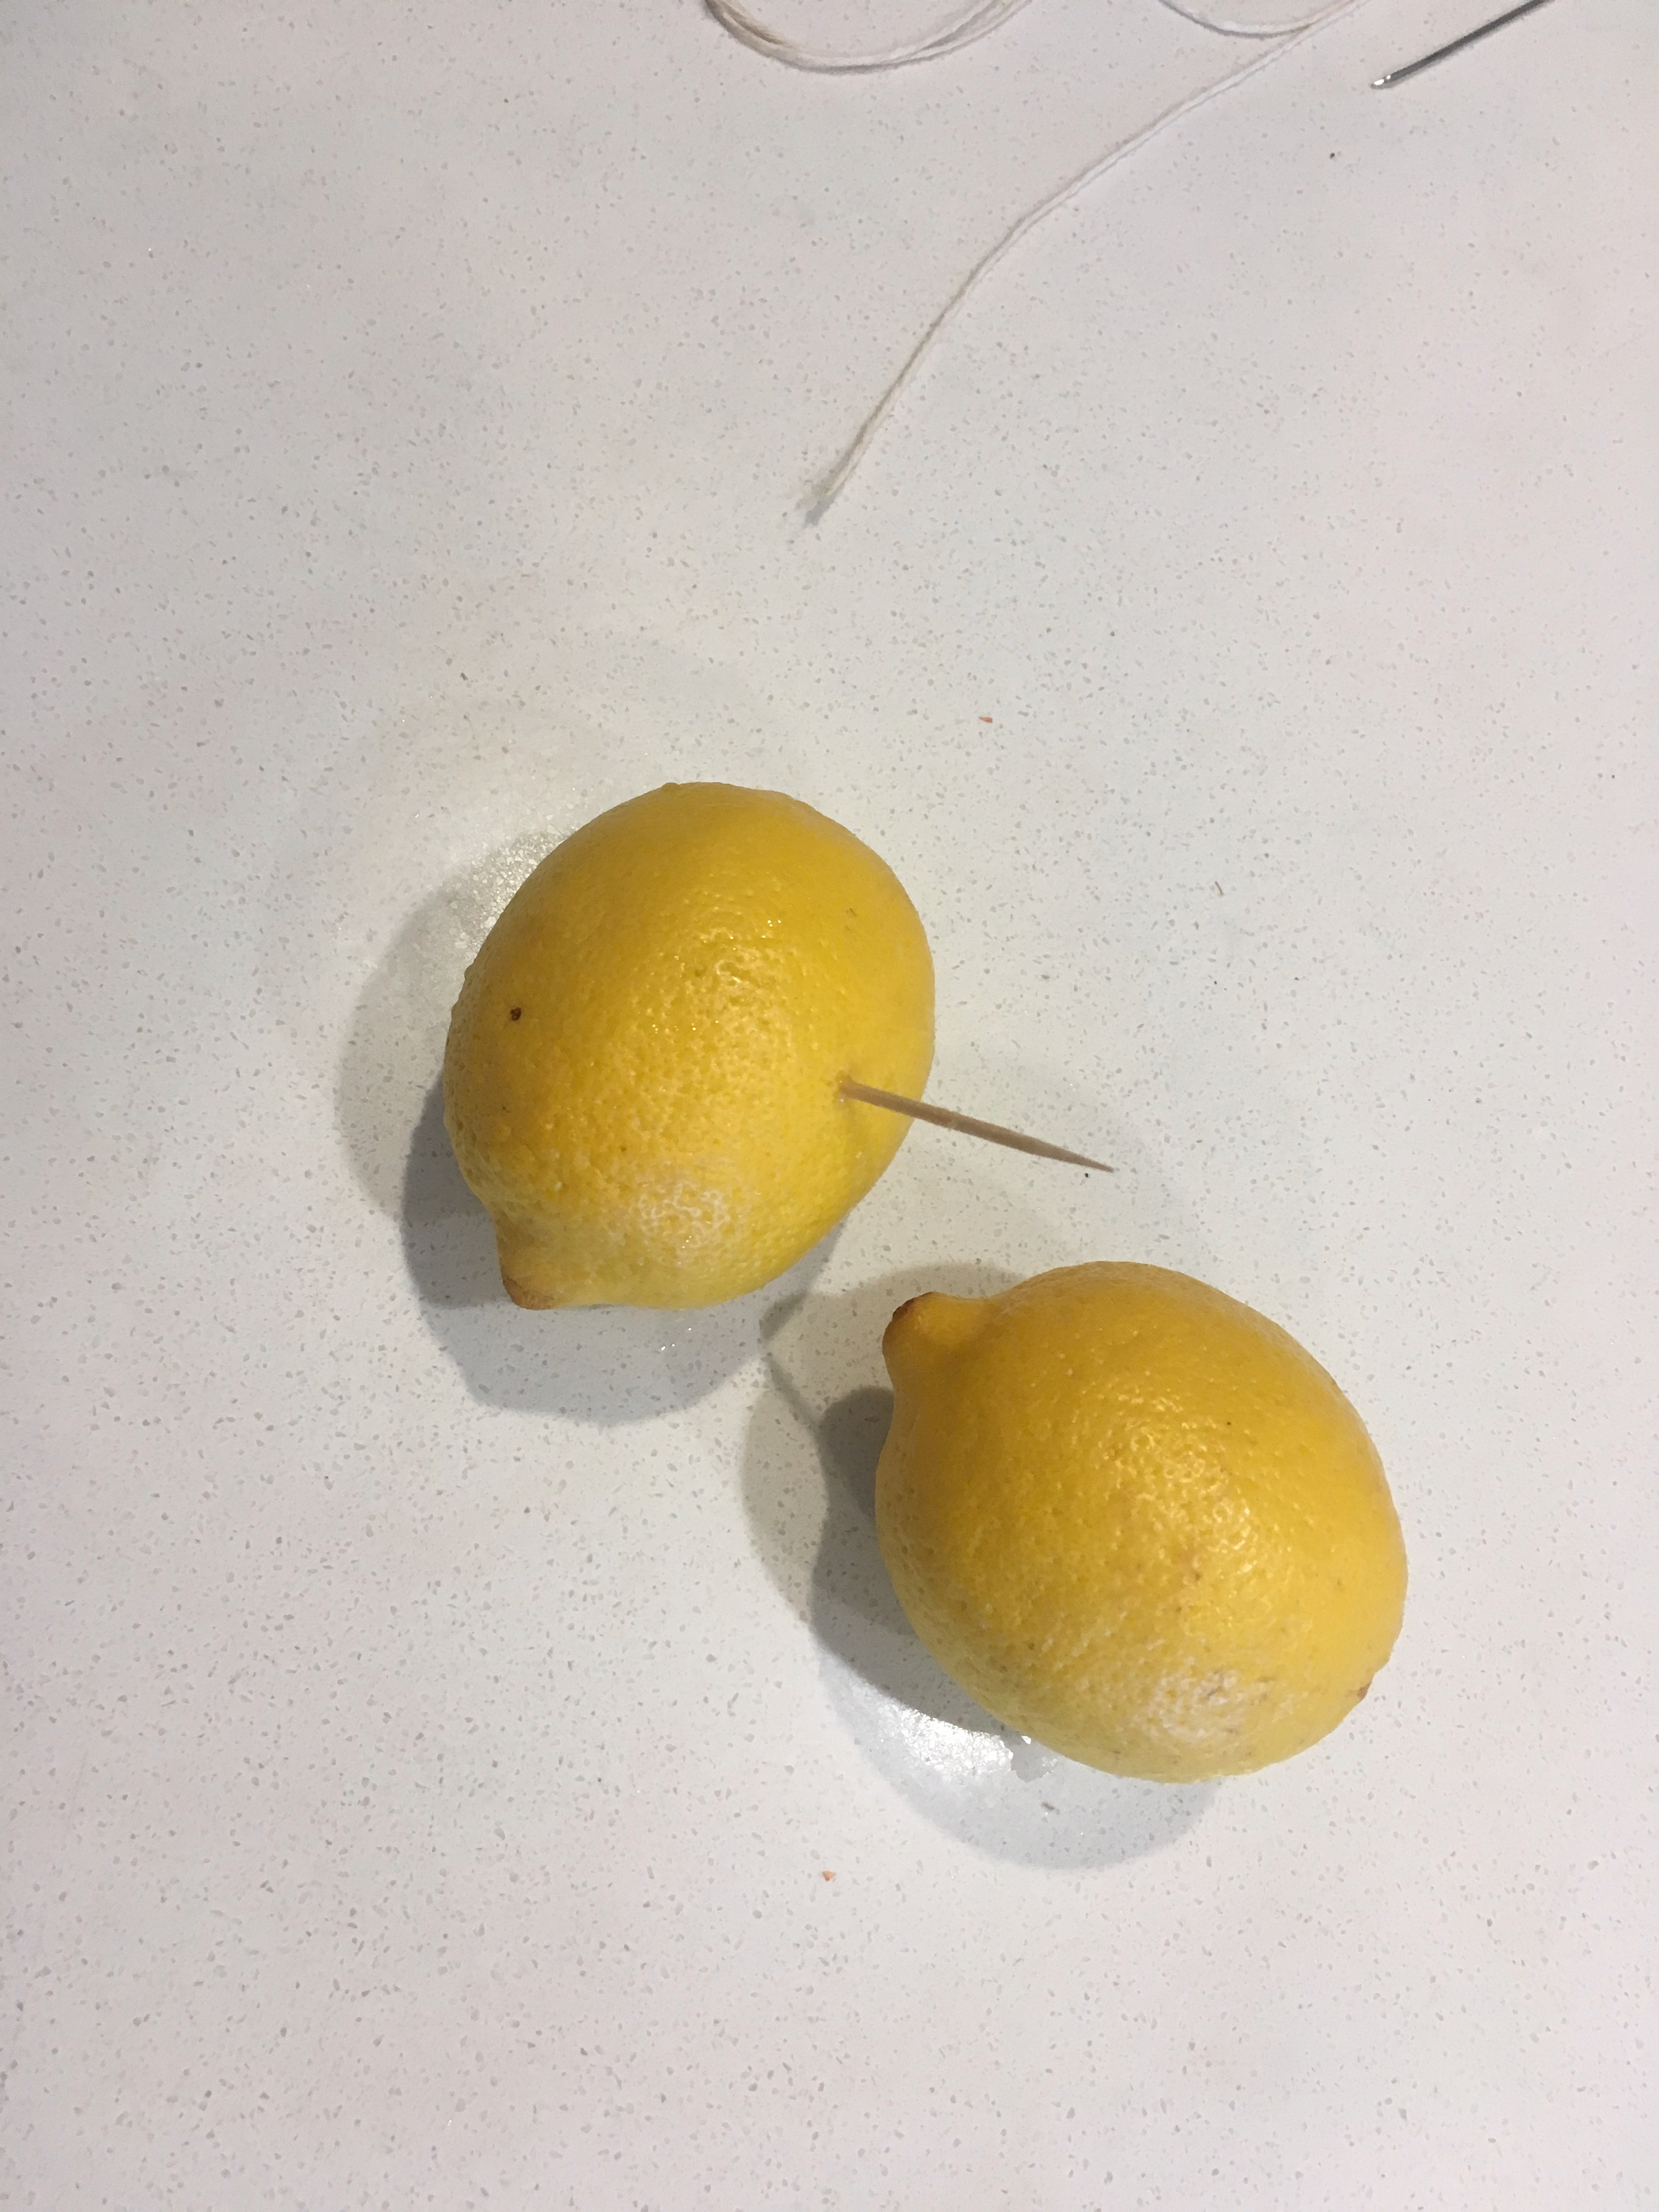
\includegraphics[width=0.25\textwidth]{\imageDir/\fileName/IMG_3212.jpg} &
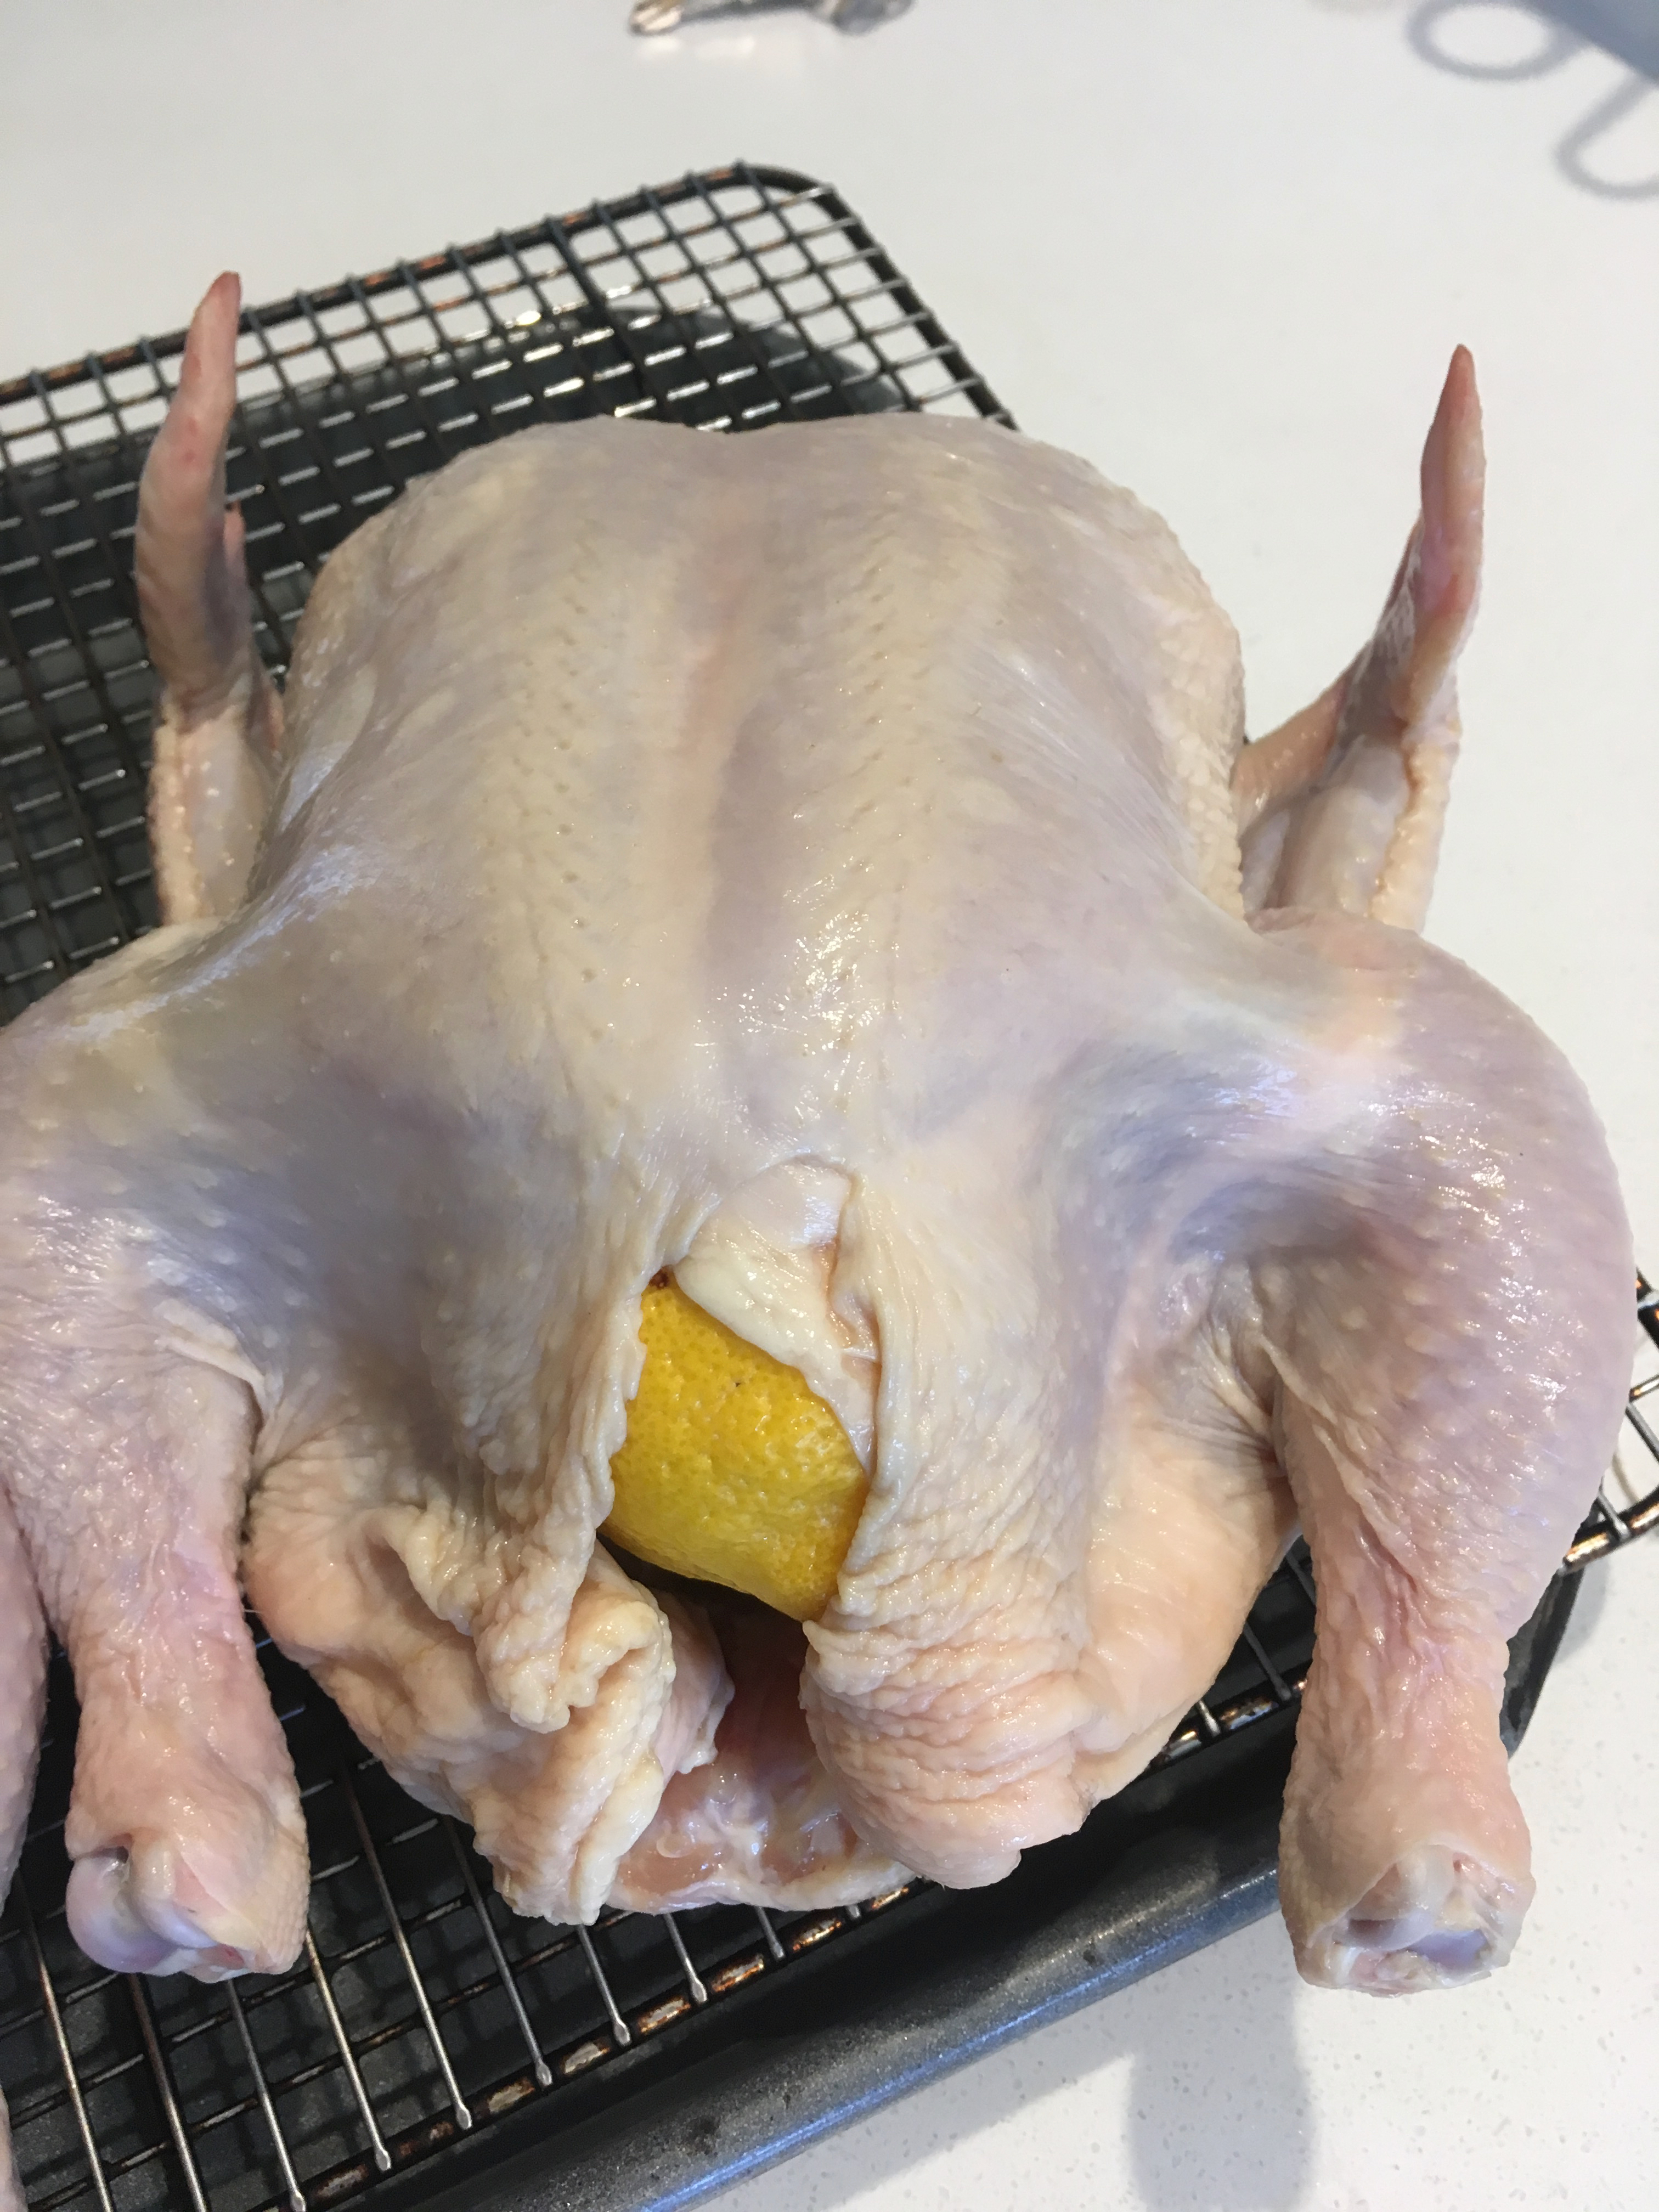
\includegraphics[width=0.25\textwidth]{\imageDir/\fileName/IMG_3213.jpg} \\
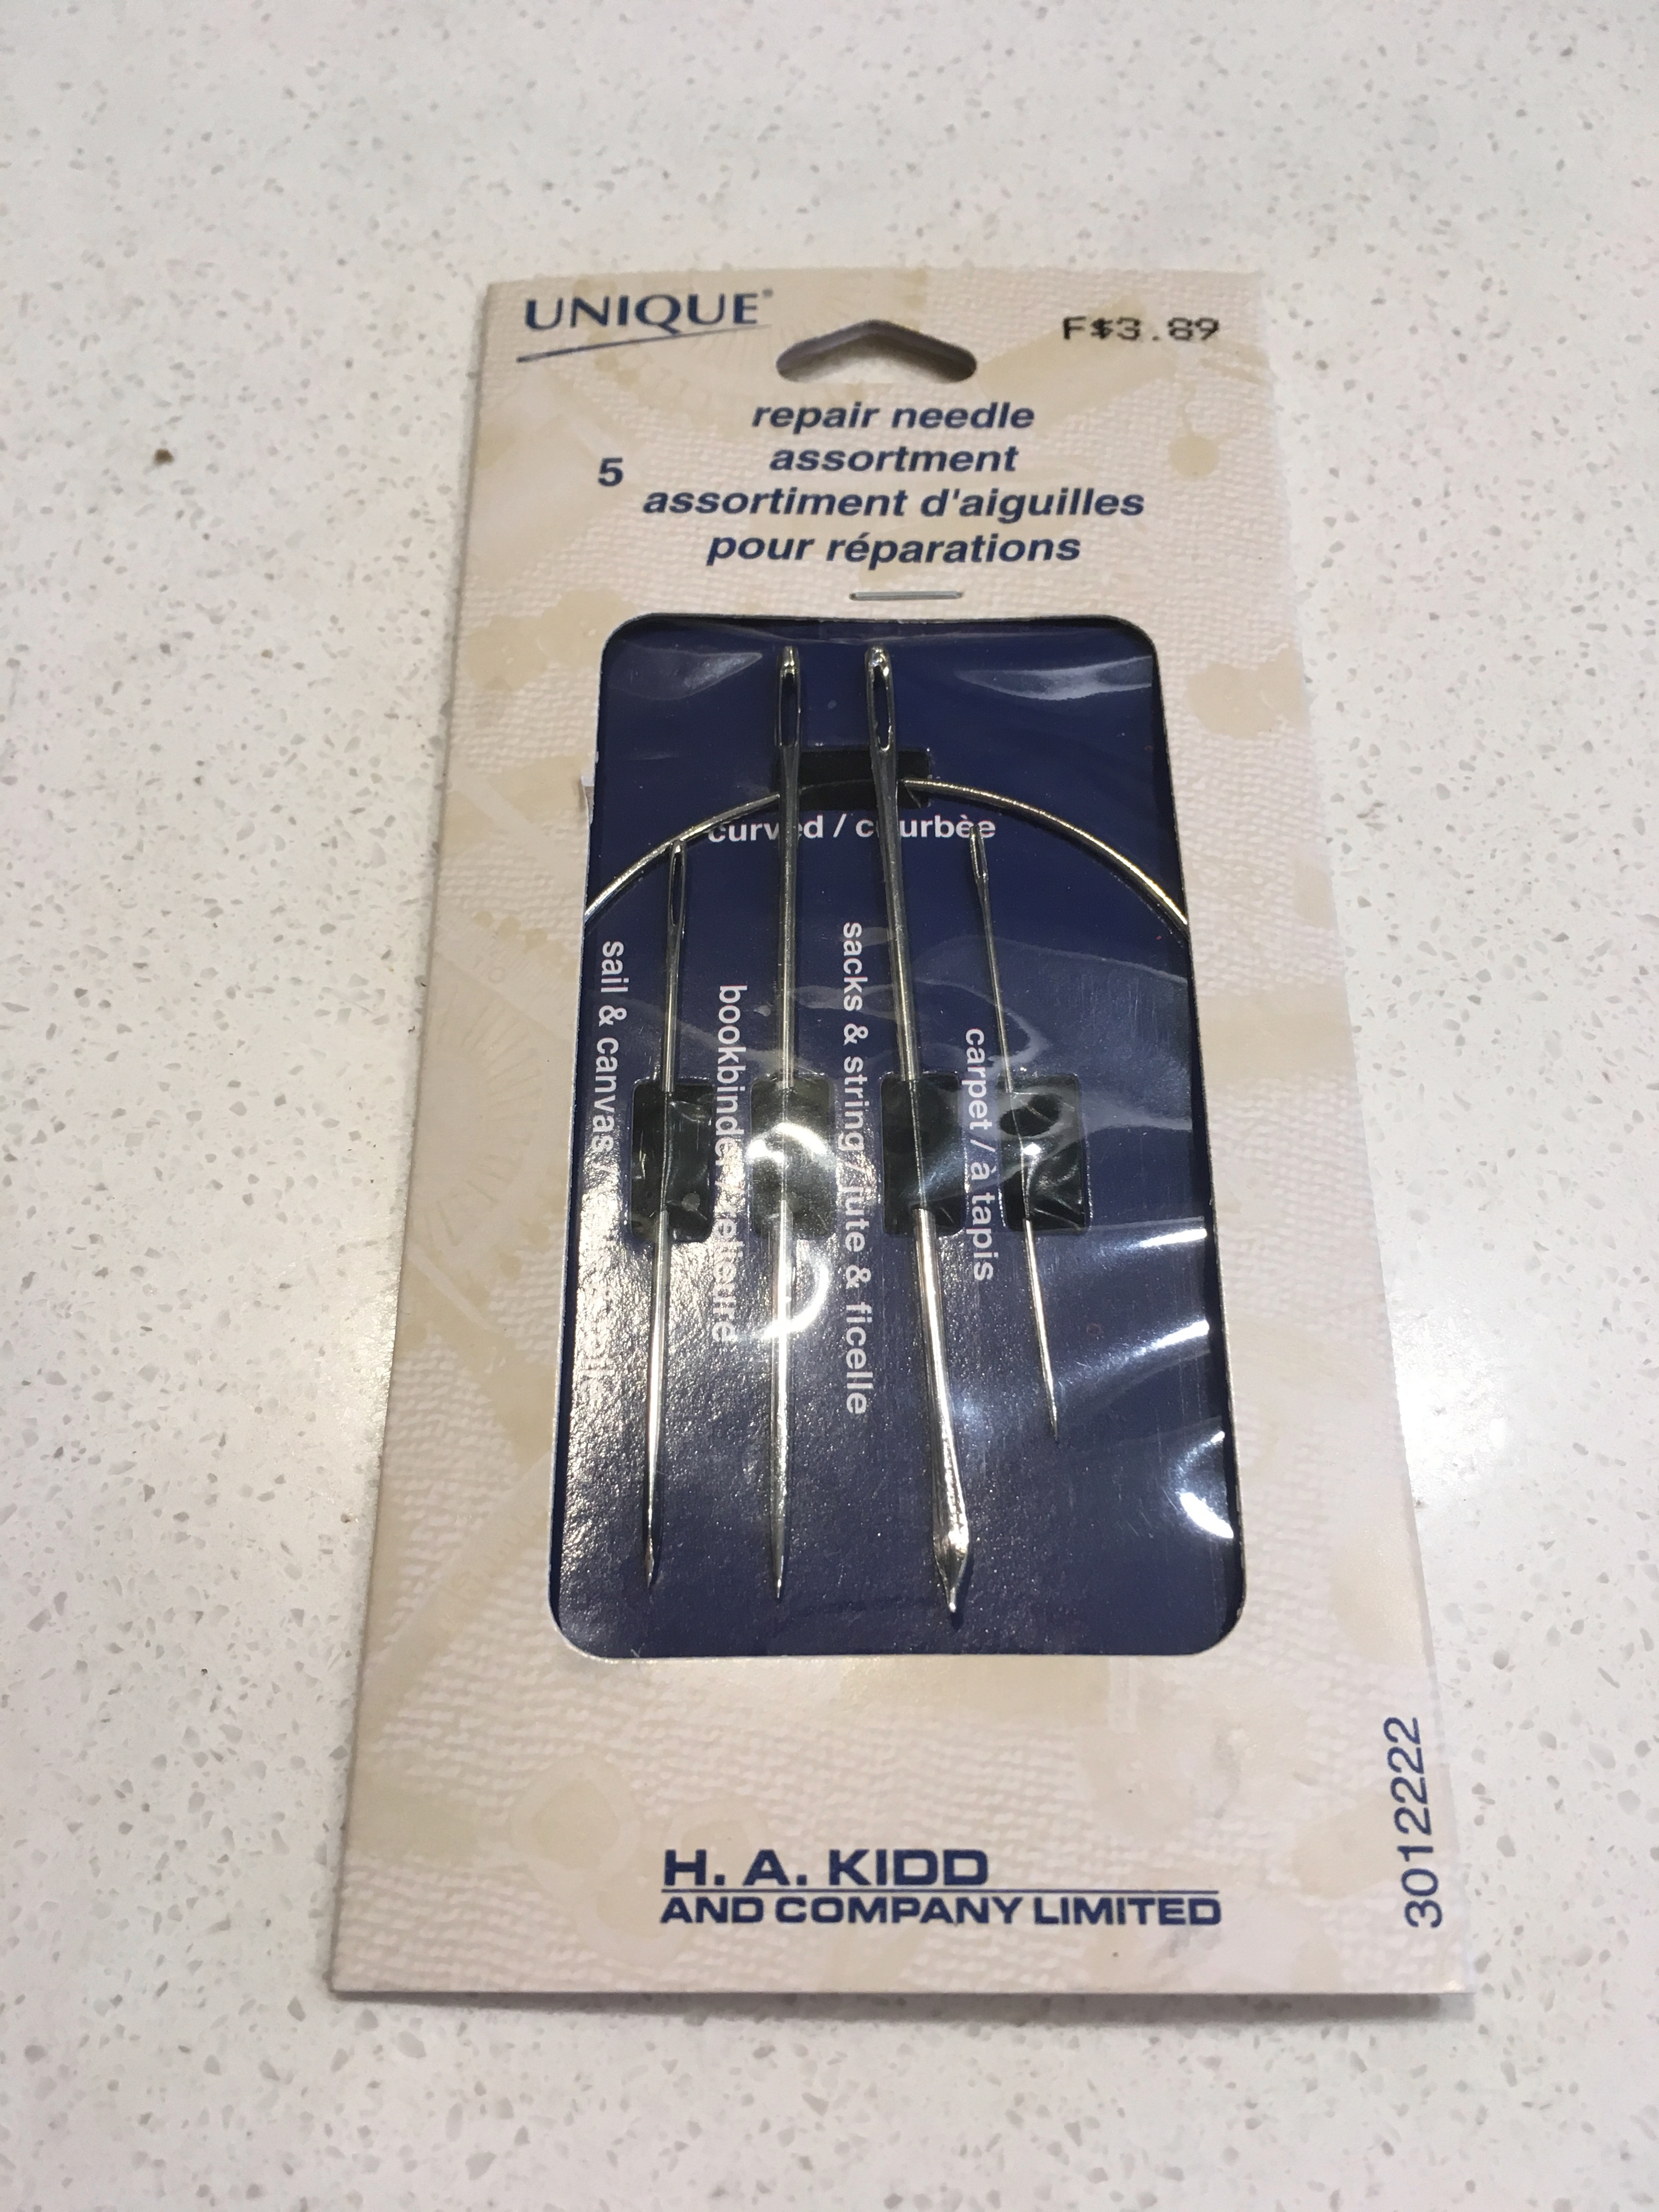
\includegraphics[width=0.25\textwidth]{\imageDir/\fileName/IMG_3206.jpg} &
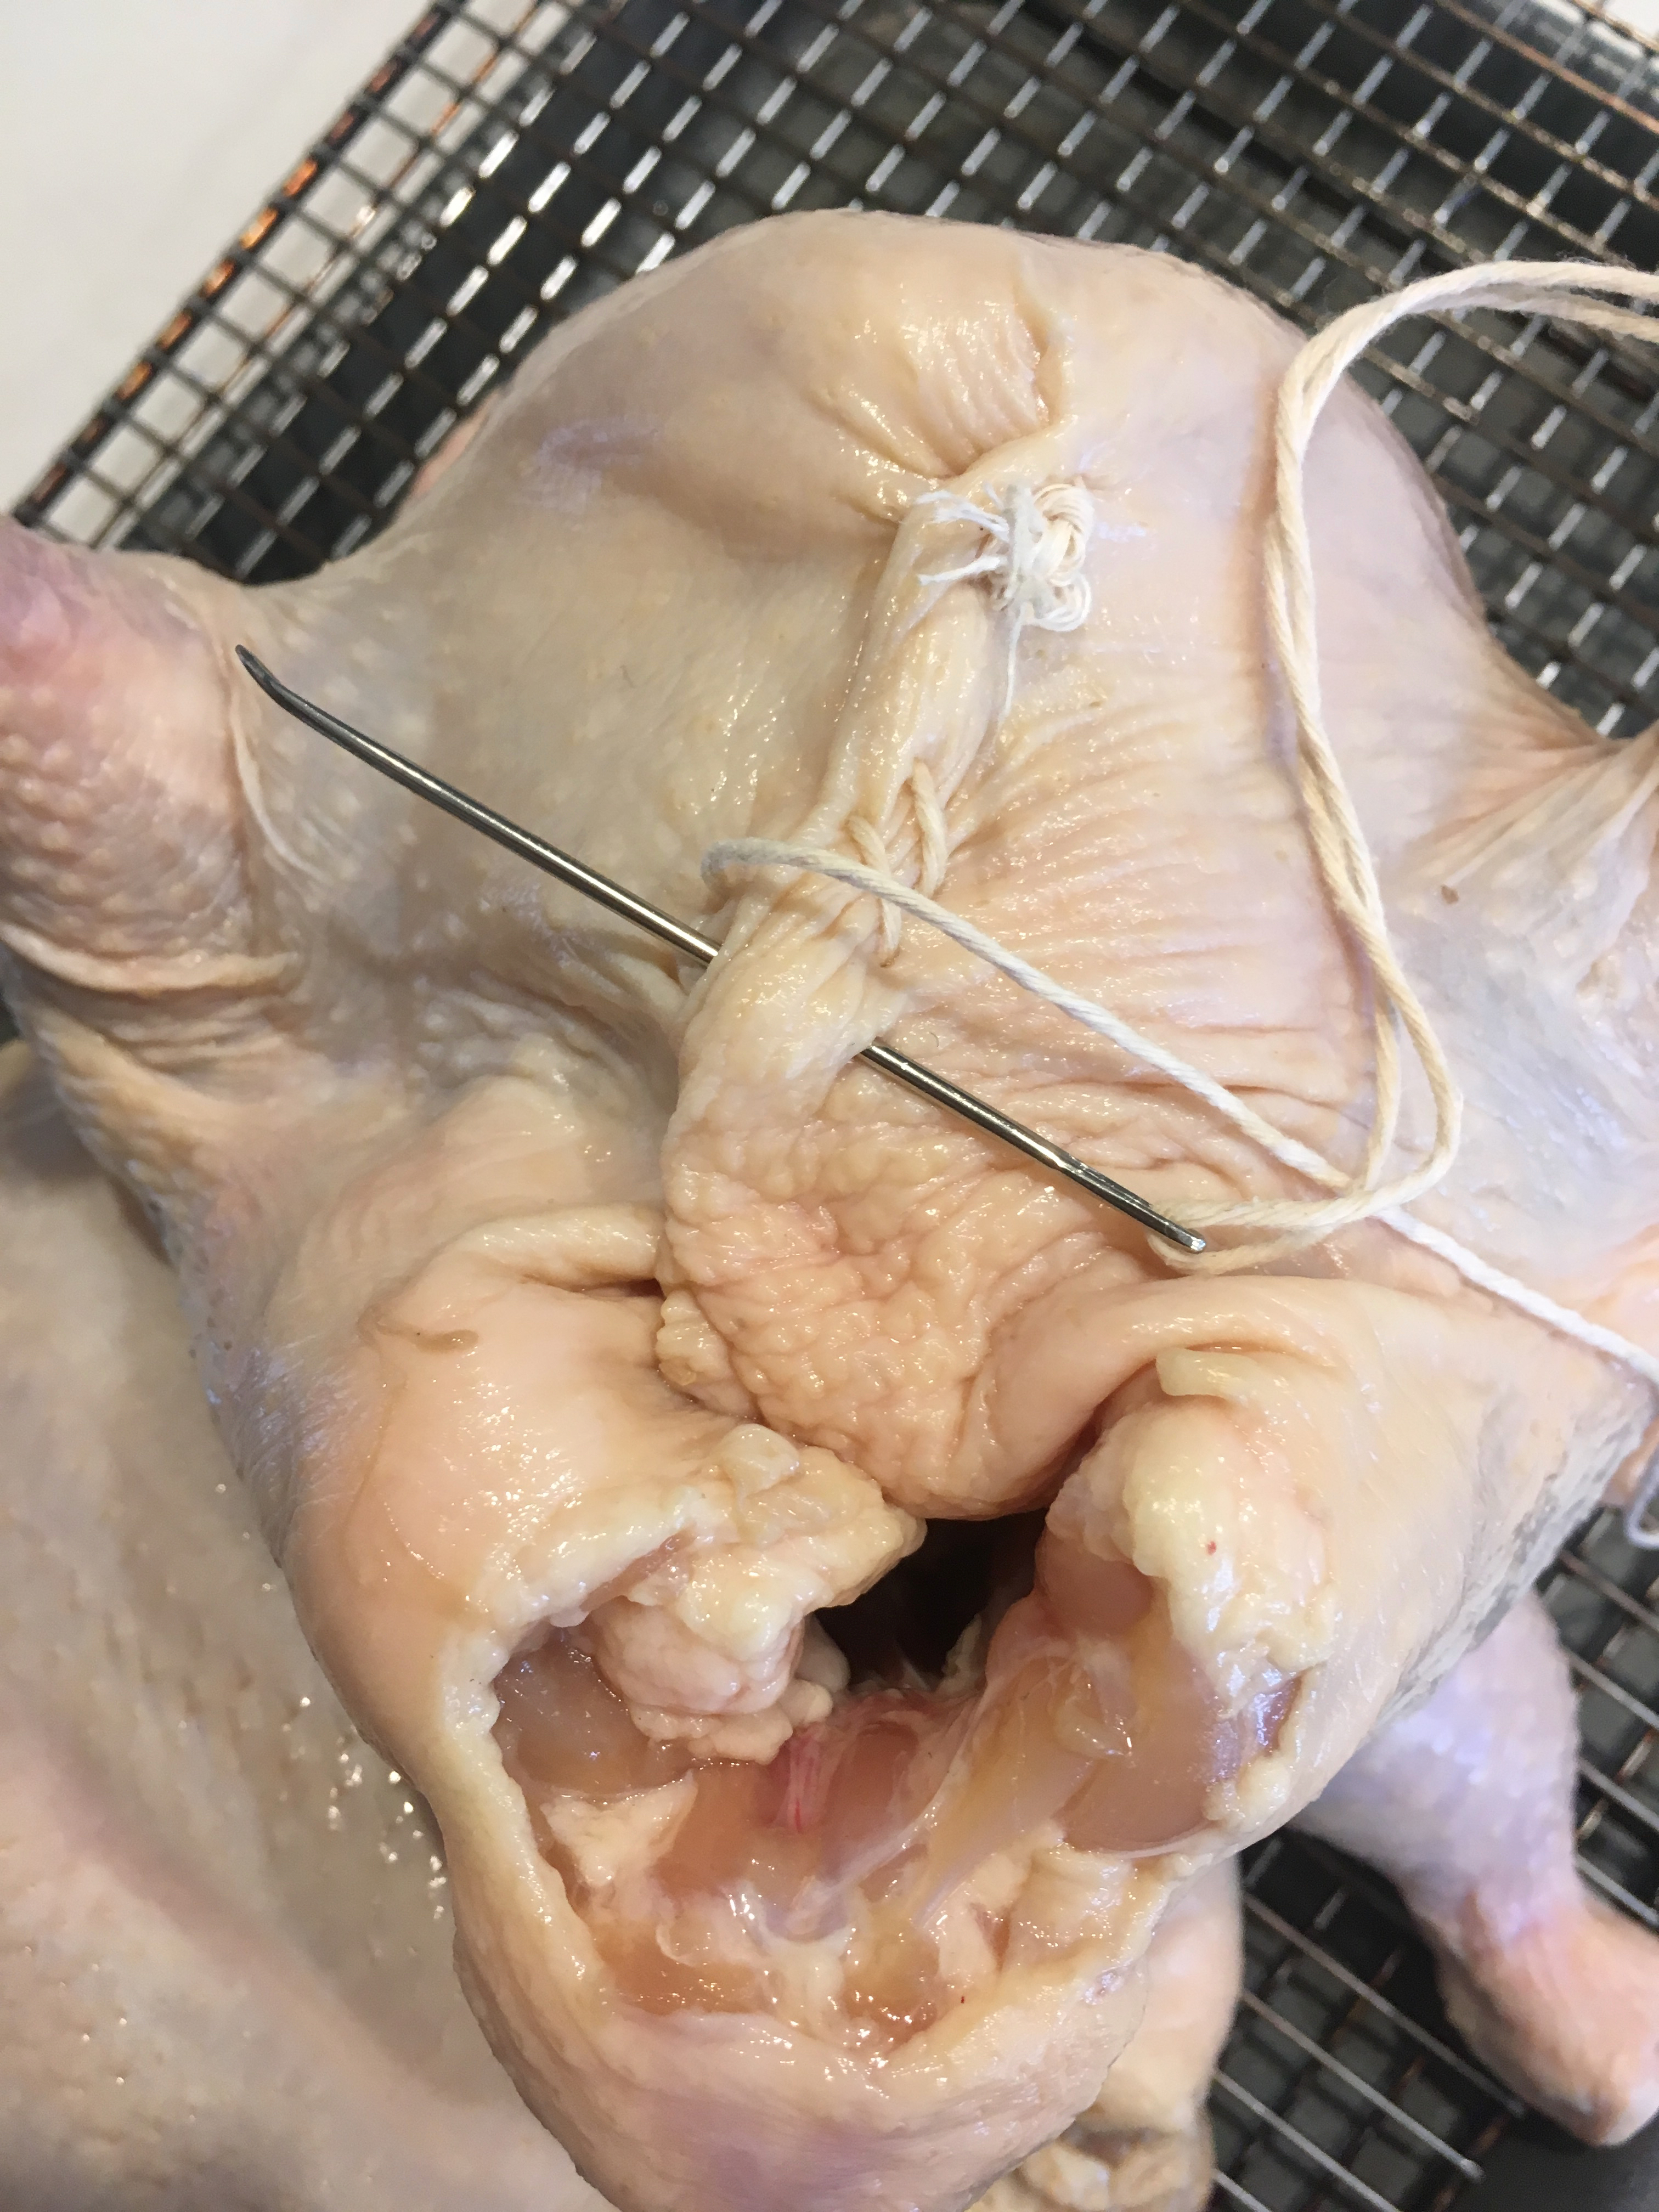
\includegraphics[width=0.25\textwidth]{\imageDir/\fileName/IMG_3214.jpg} &
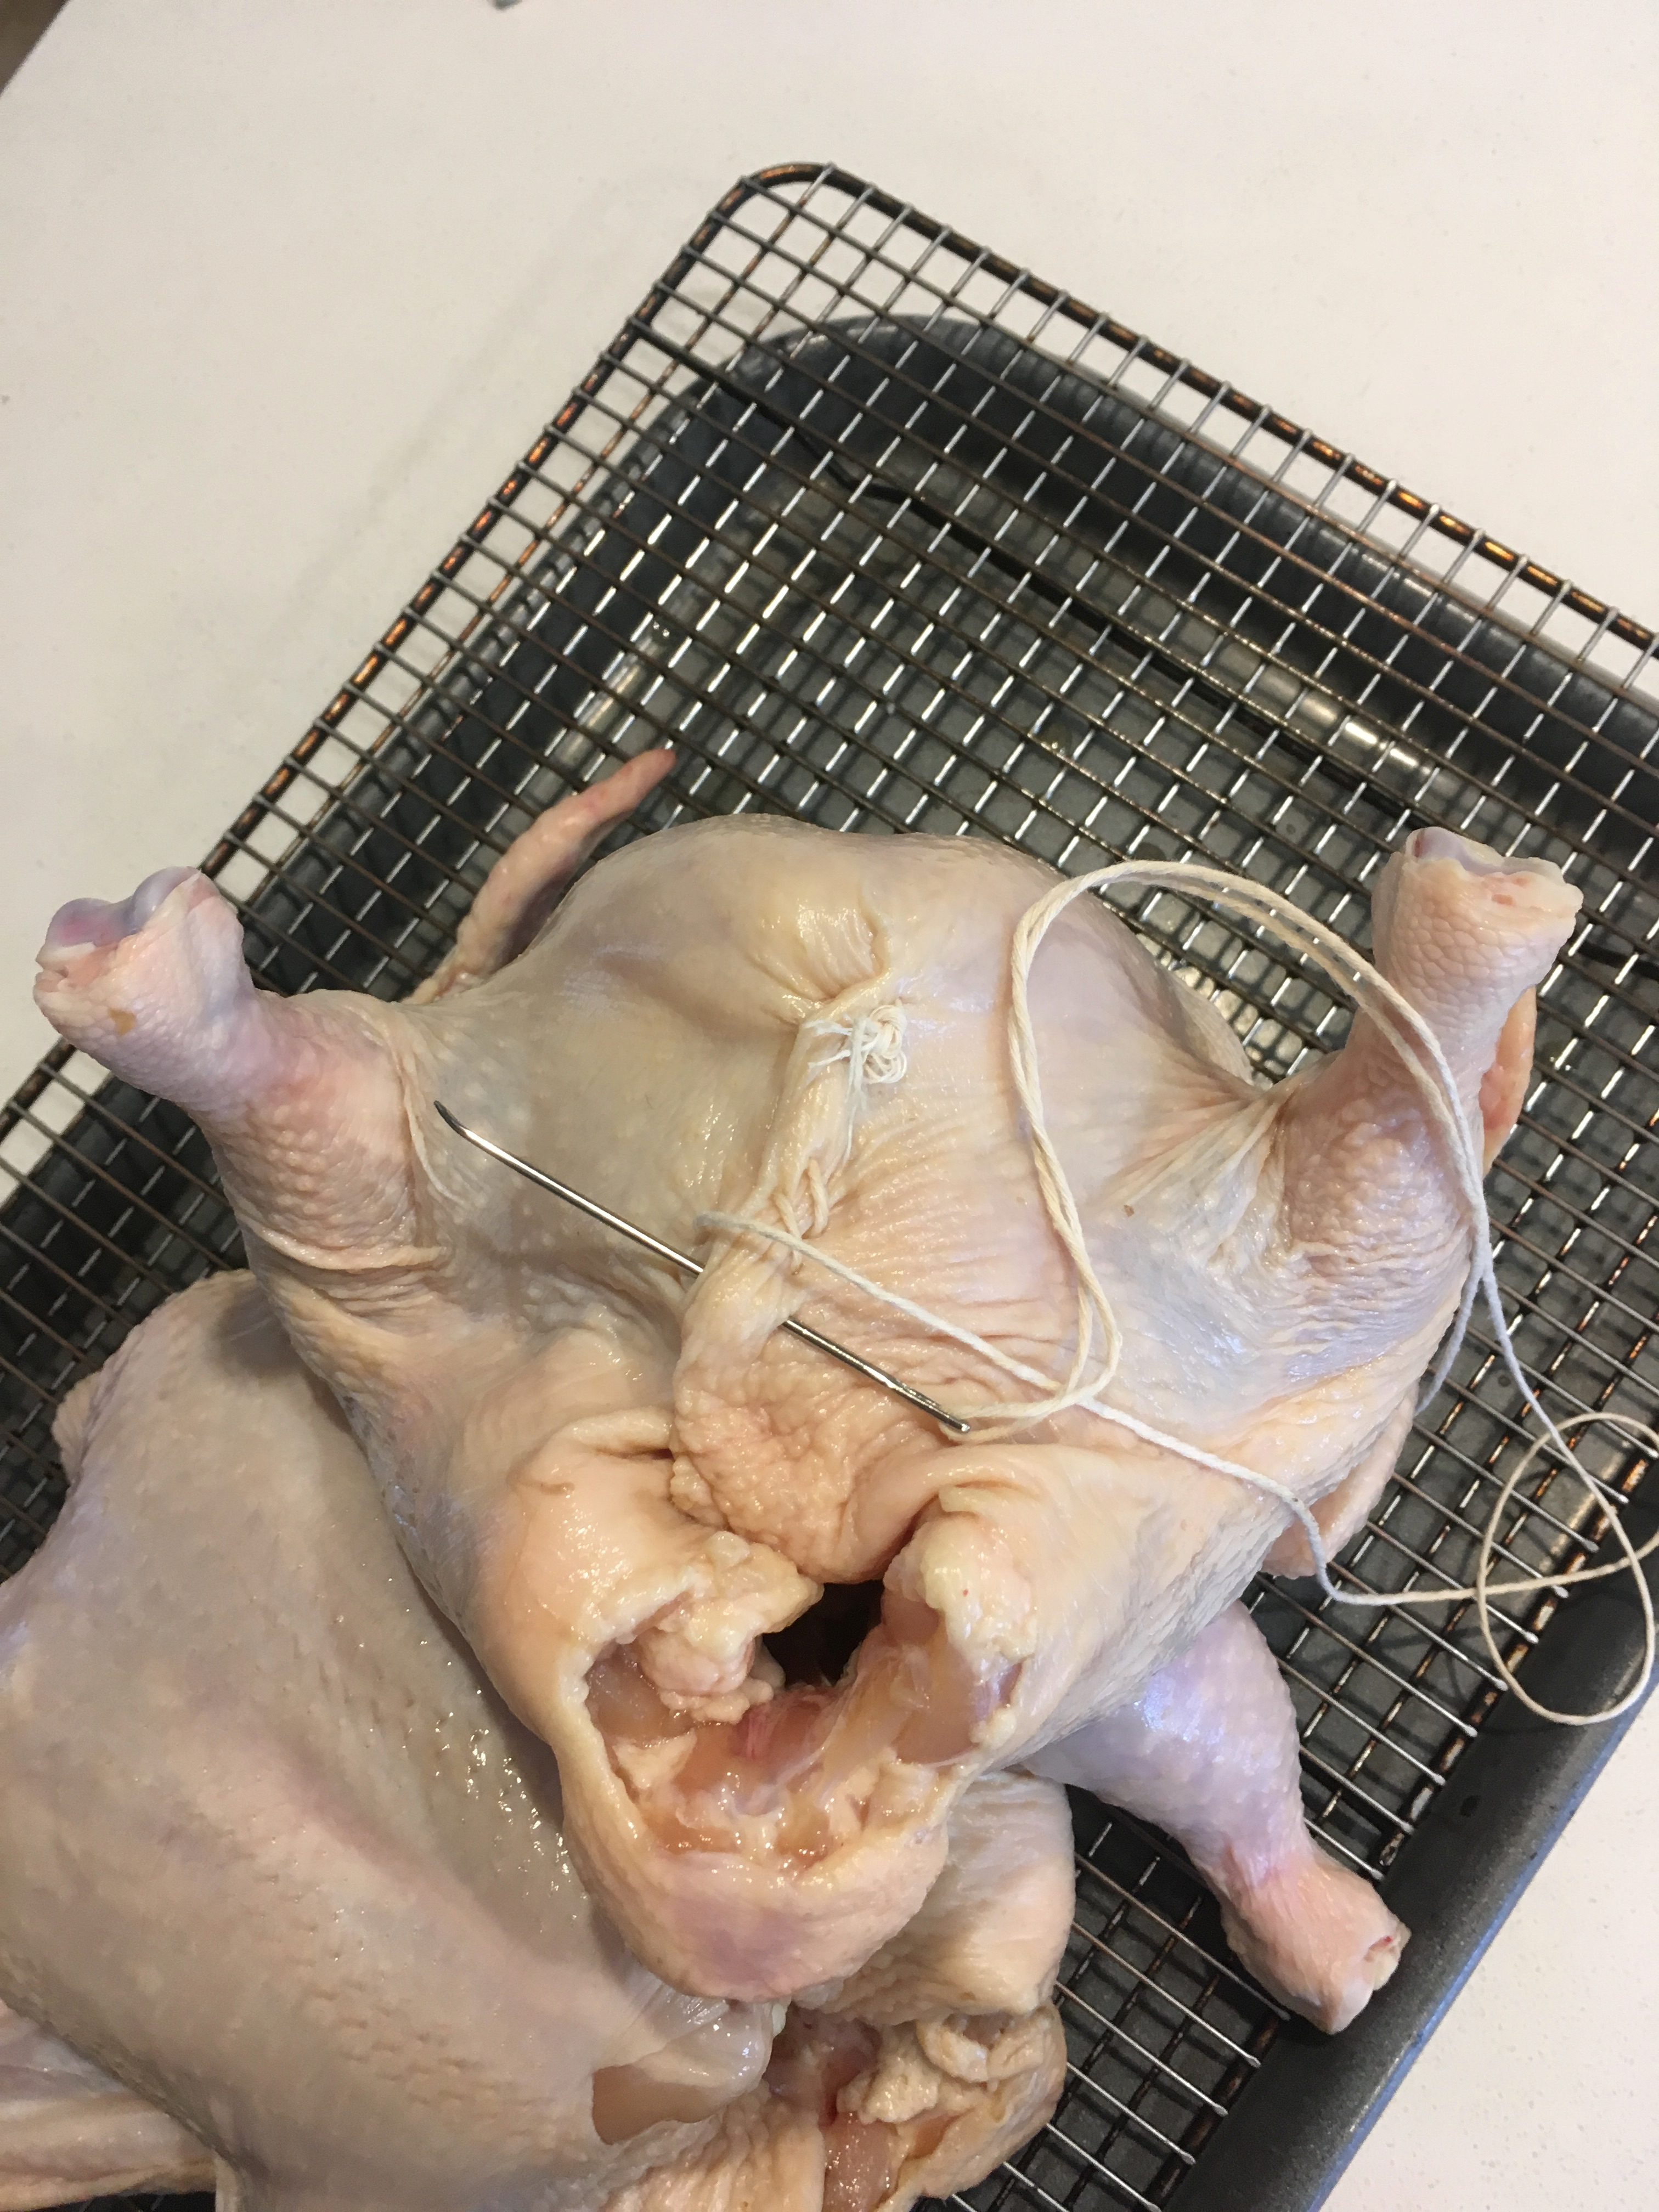
\includegraphics[width=0.25\textwidth]{\imageDir/\fileName/IMG_3216.jpg} \\
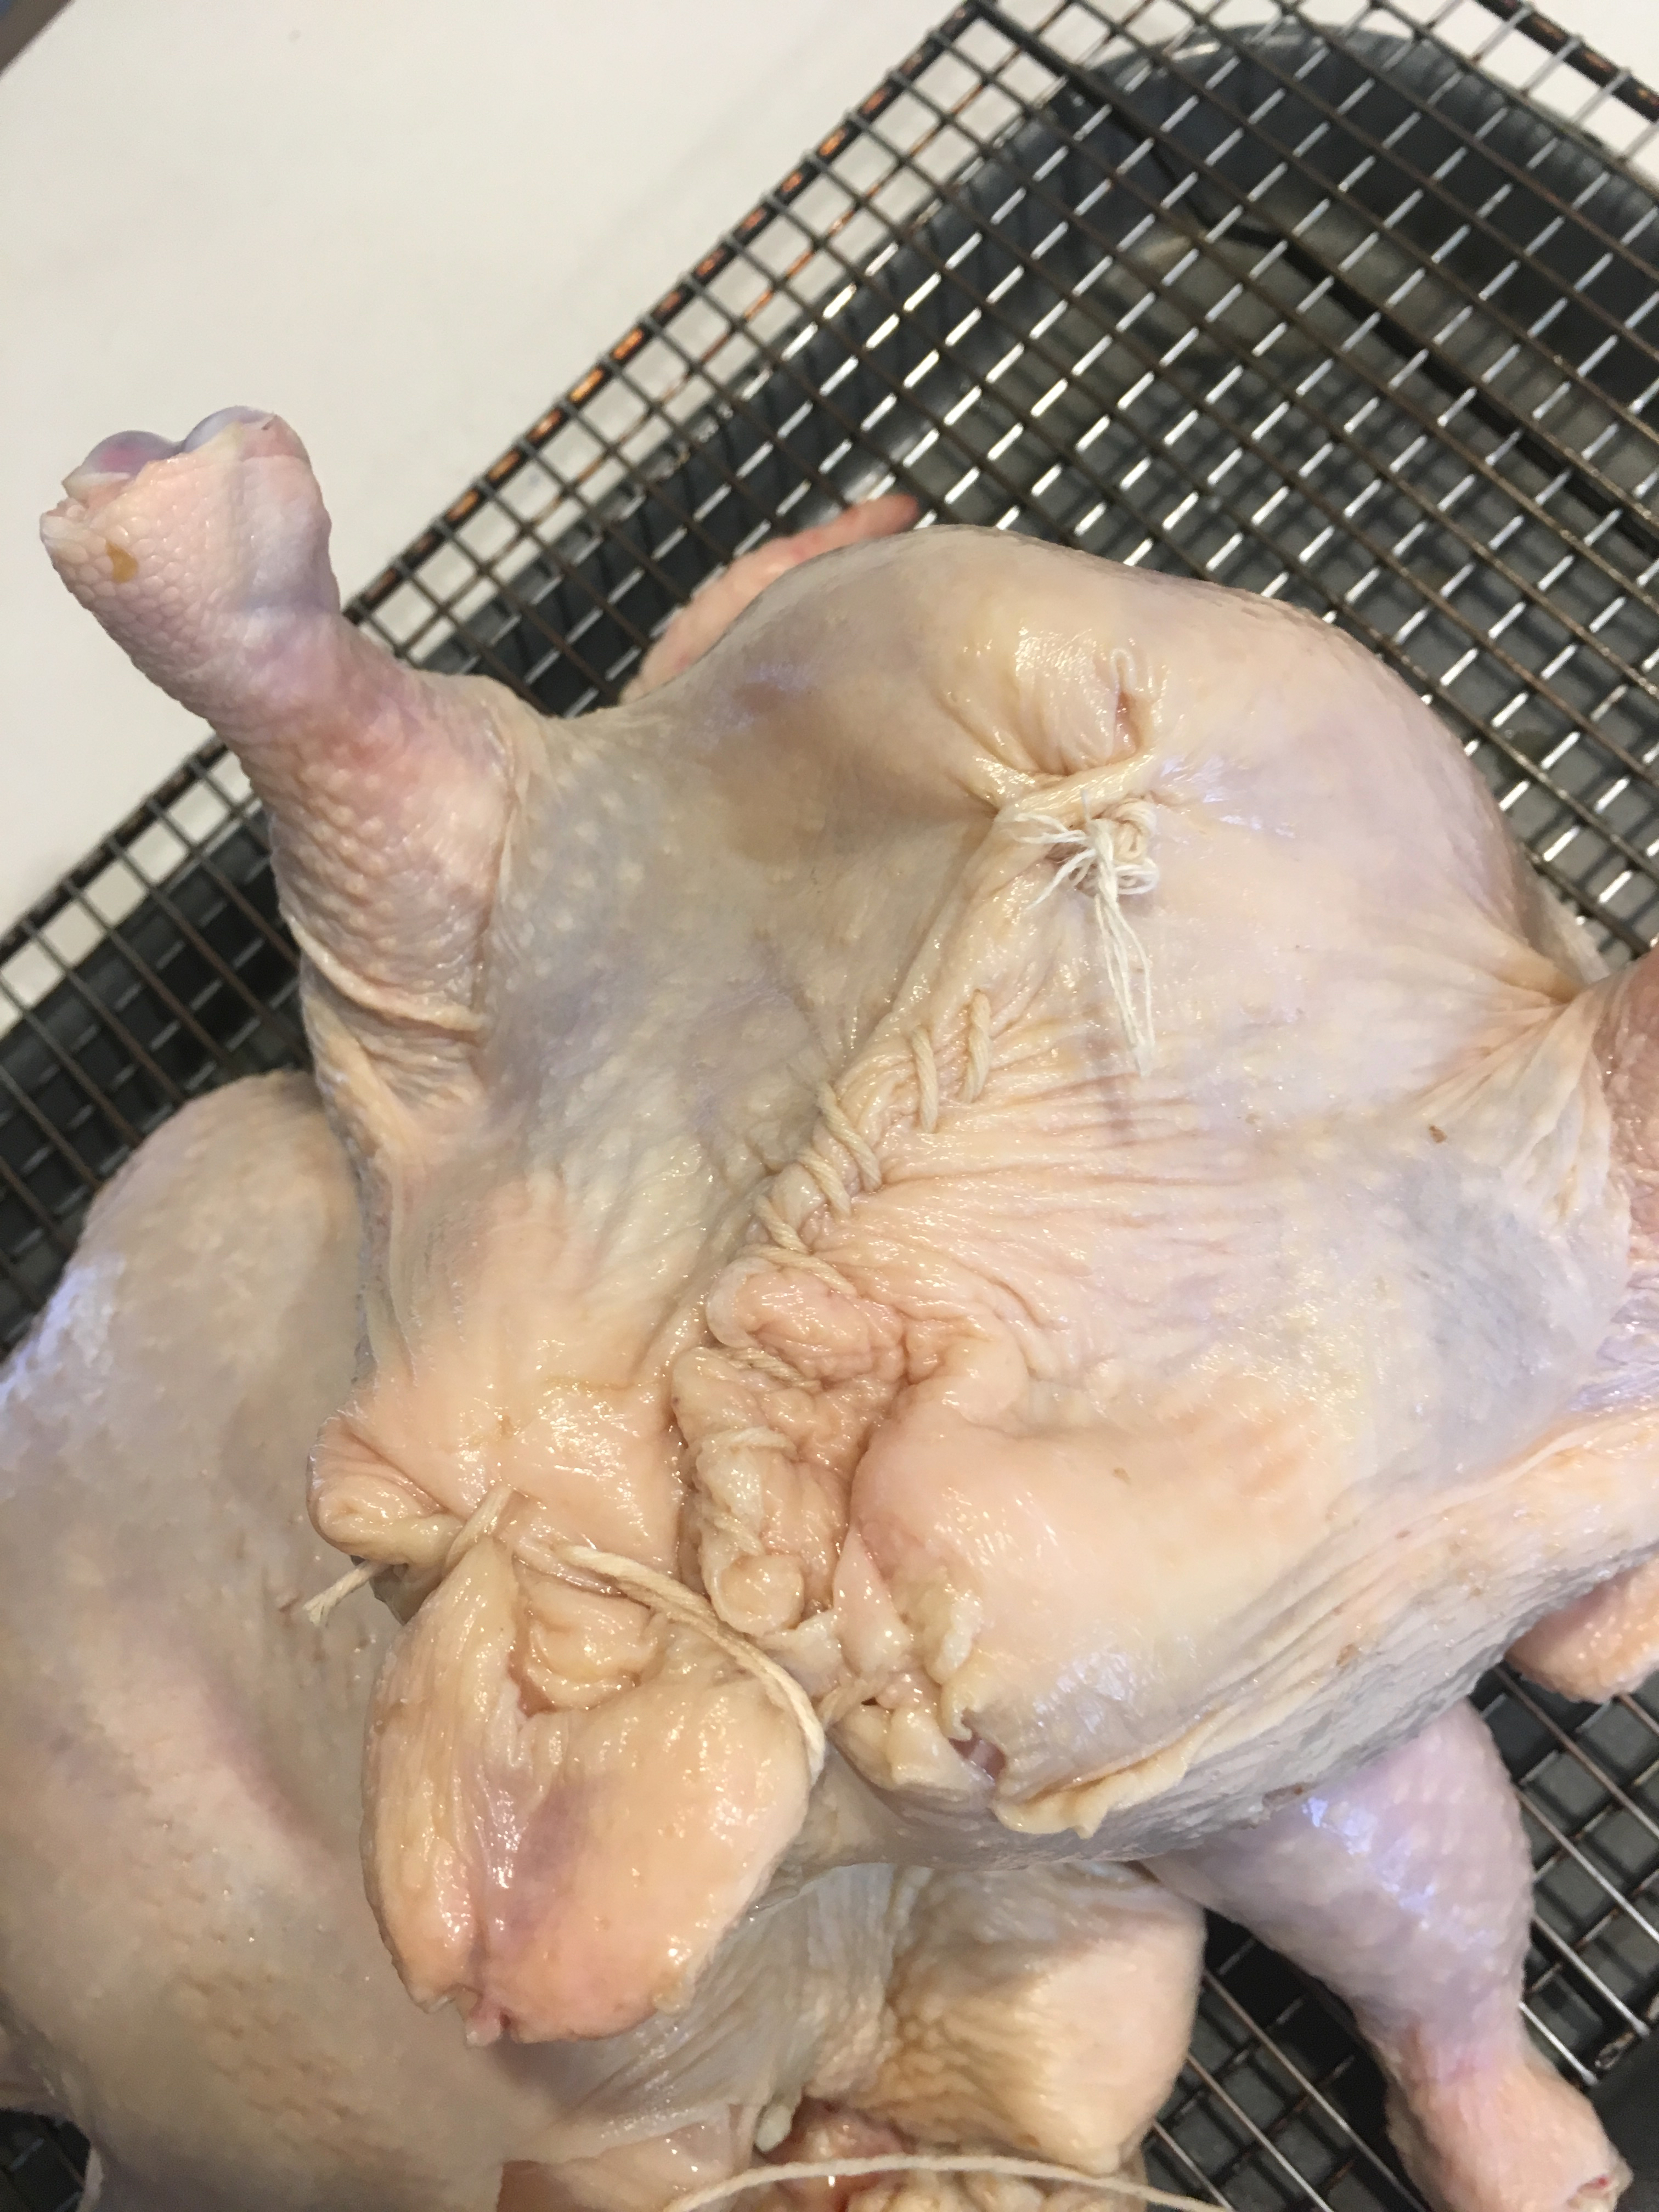
\includegraphics[width=0.25\textwidth]{\imageDir/\fileName/IMG_3217.jpg} &
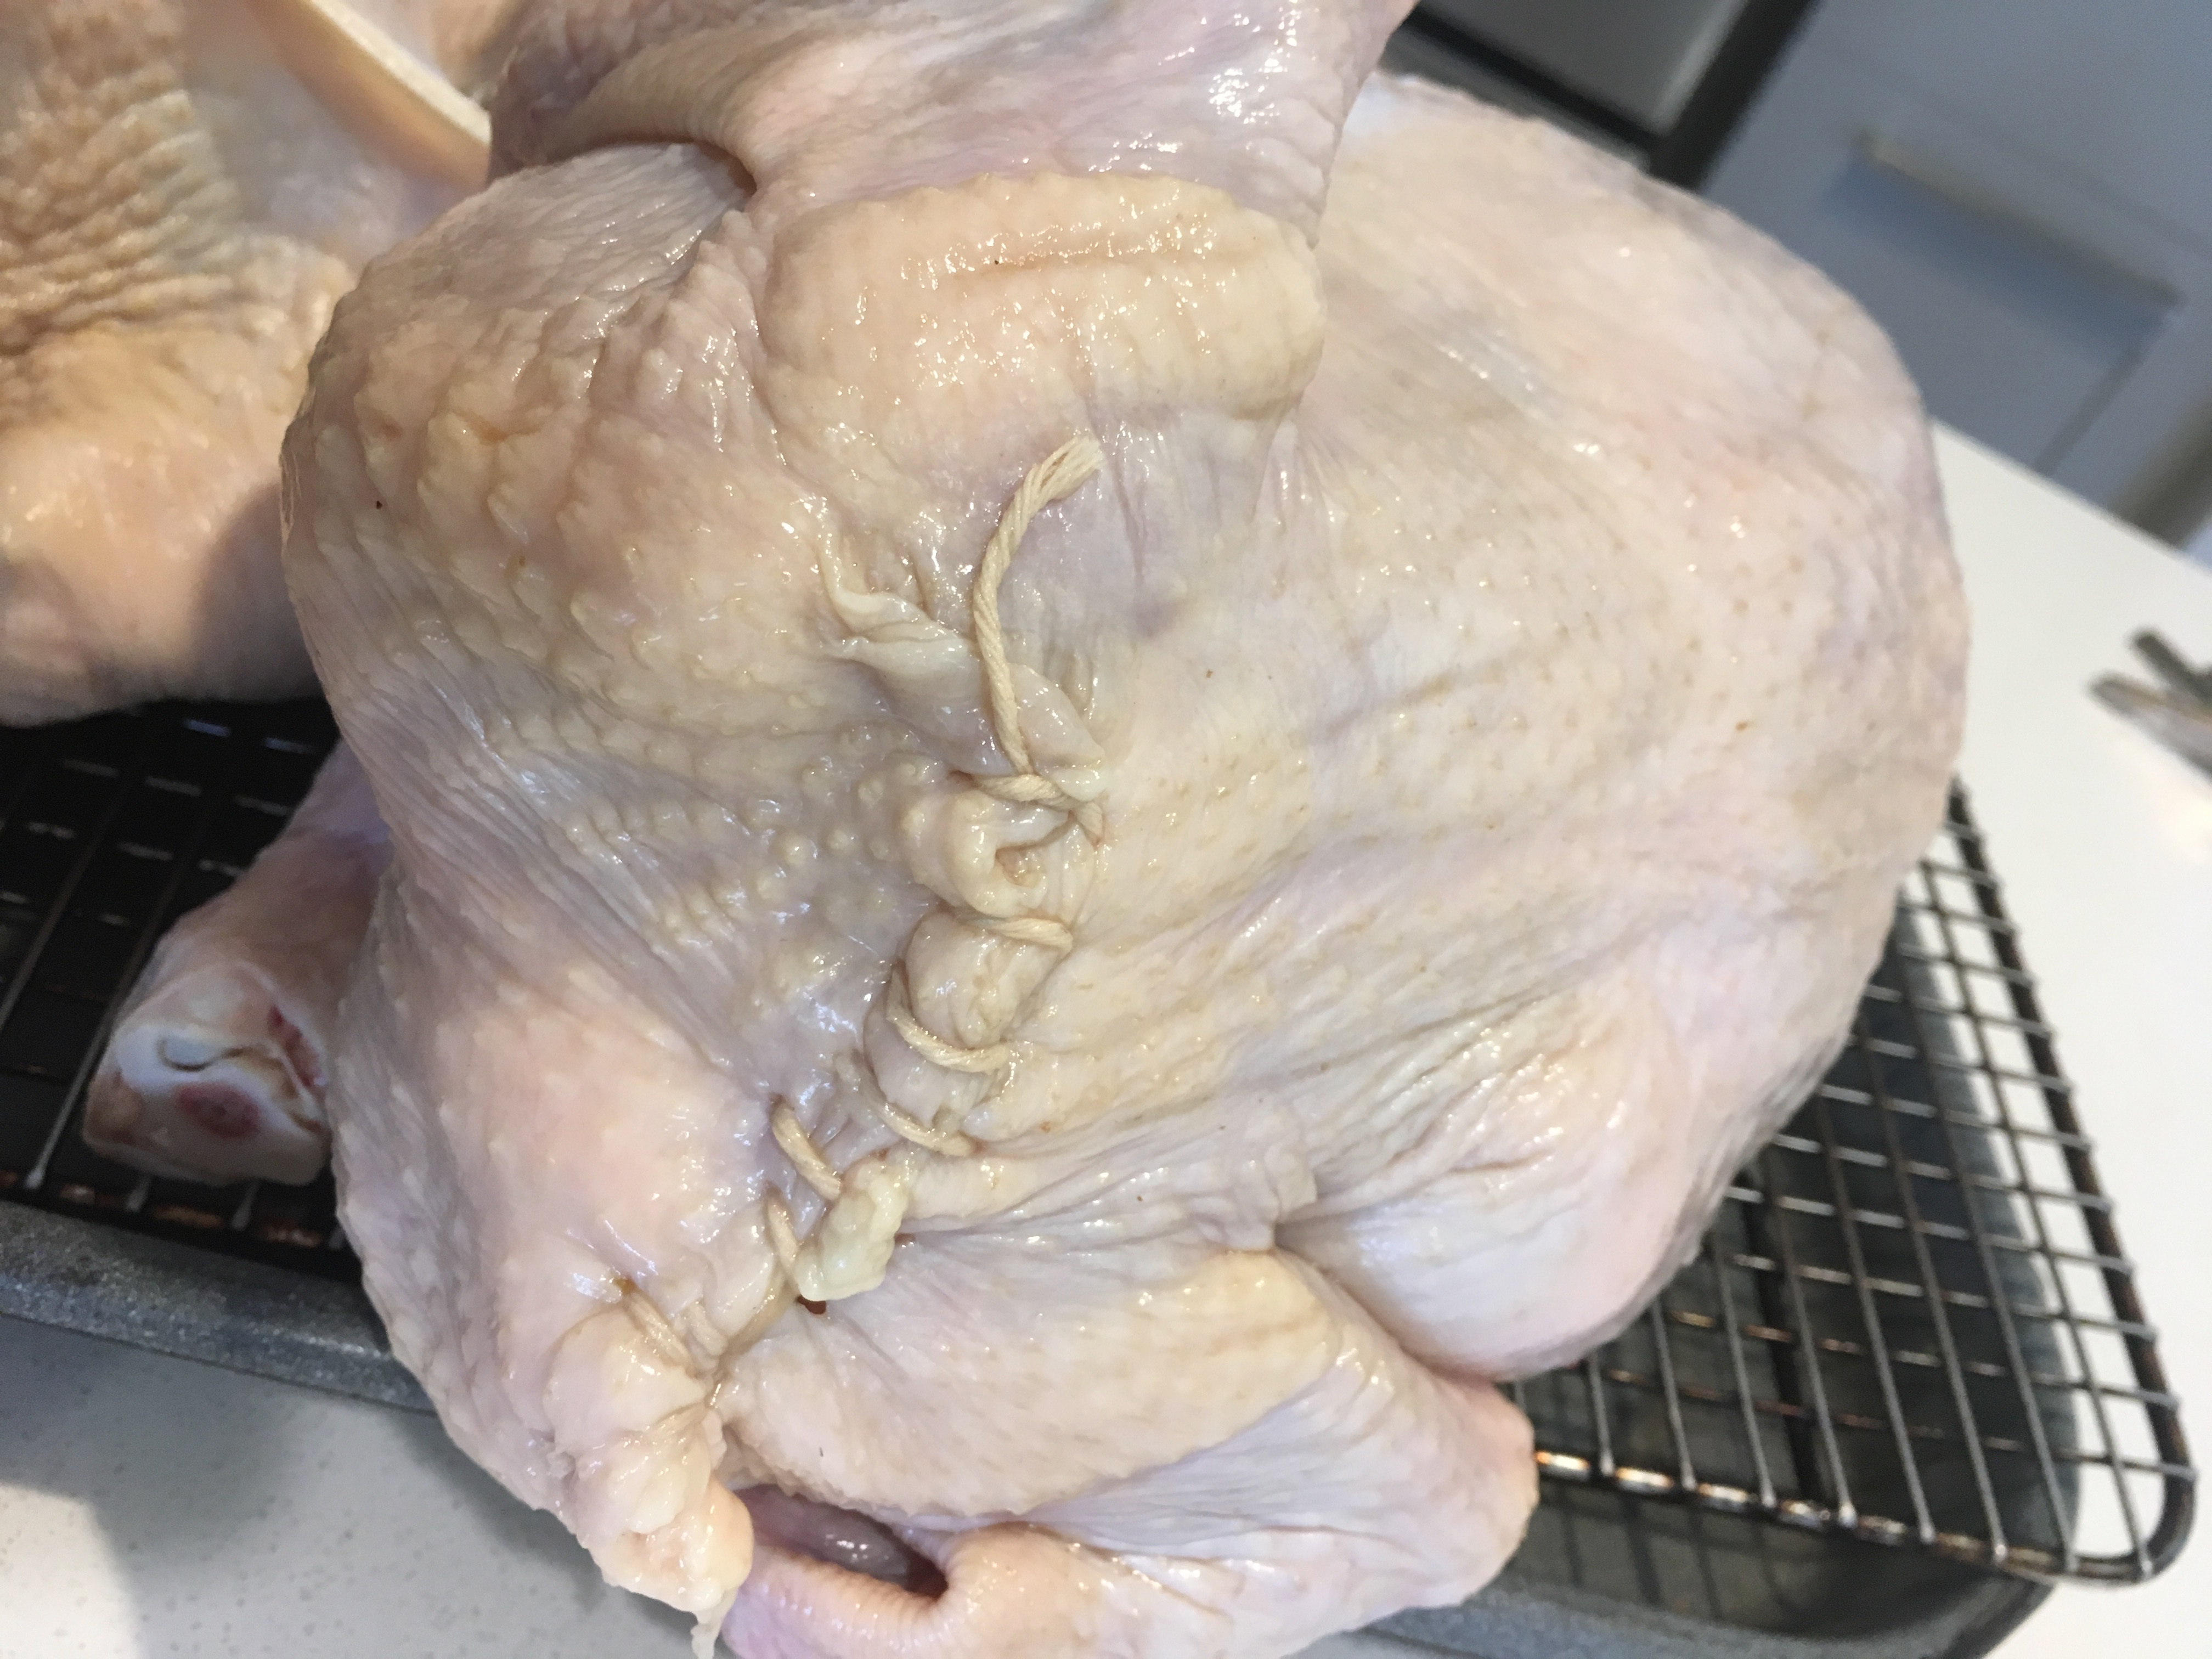
\includegraphics[width=0.25\textwidth]{\imageDir/\fileName/IMG_3218.jpg} &
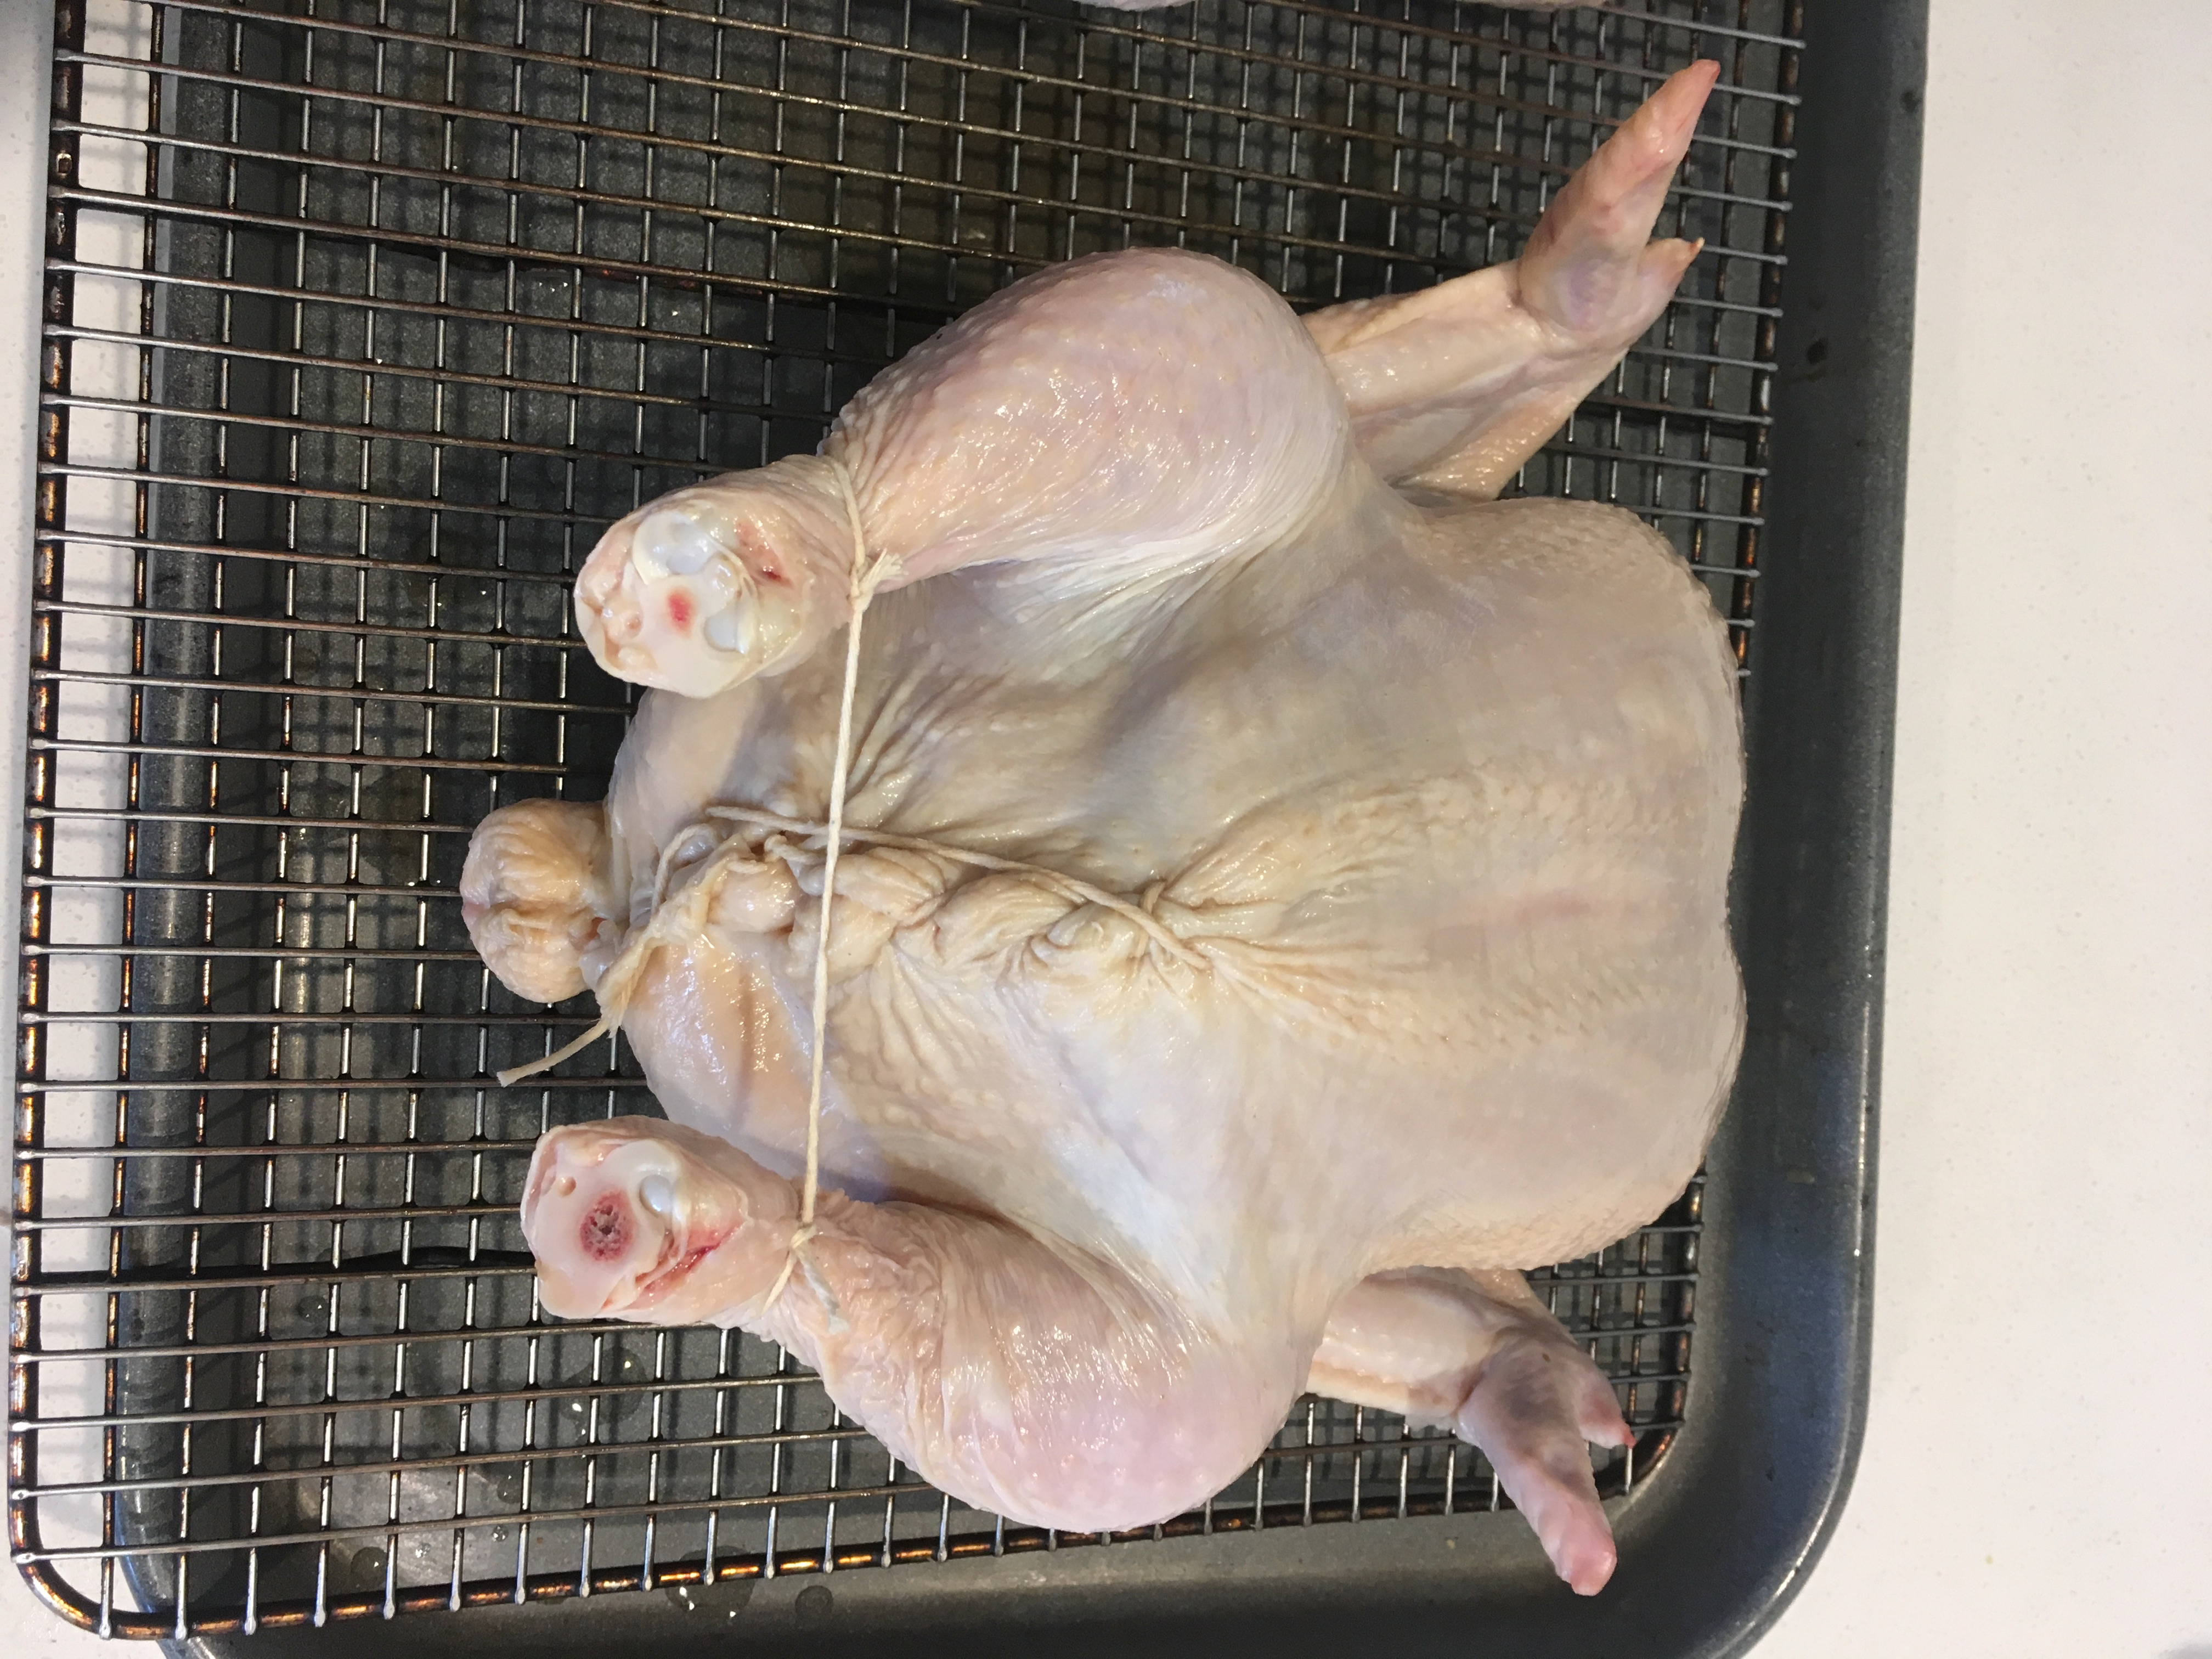
\includegraphics[width=0.25\textwidth]{\imageDir/\fileName/IMG_3219.jpg} \\
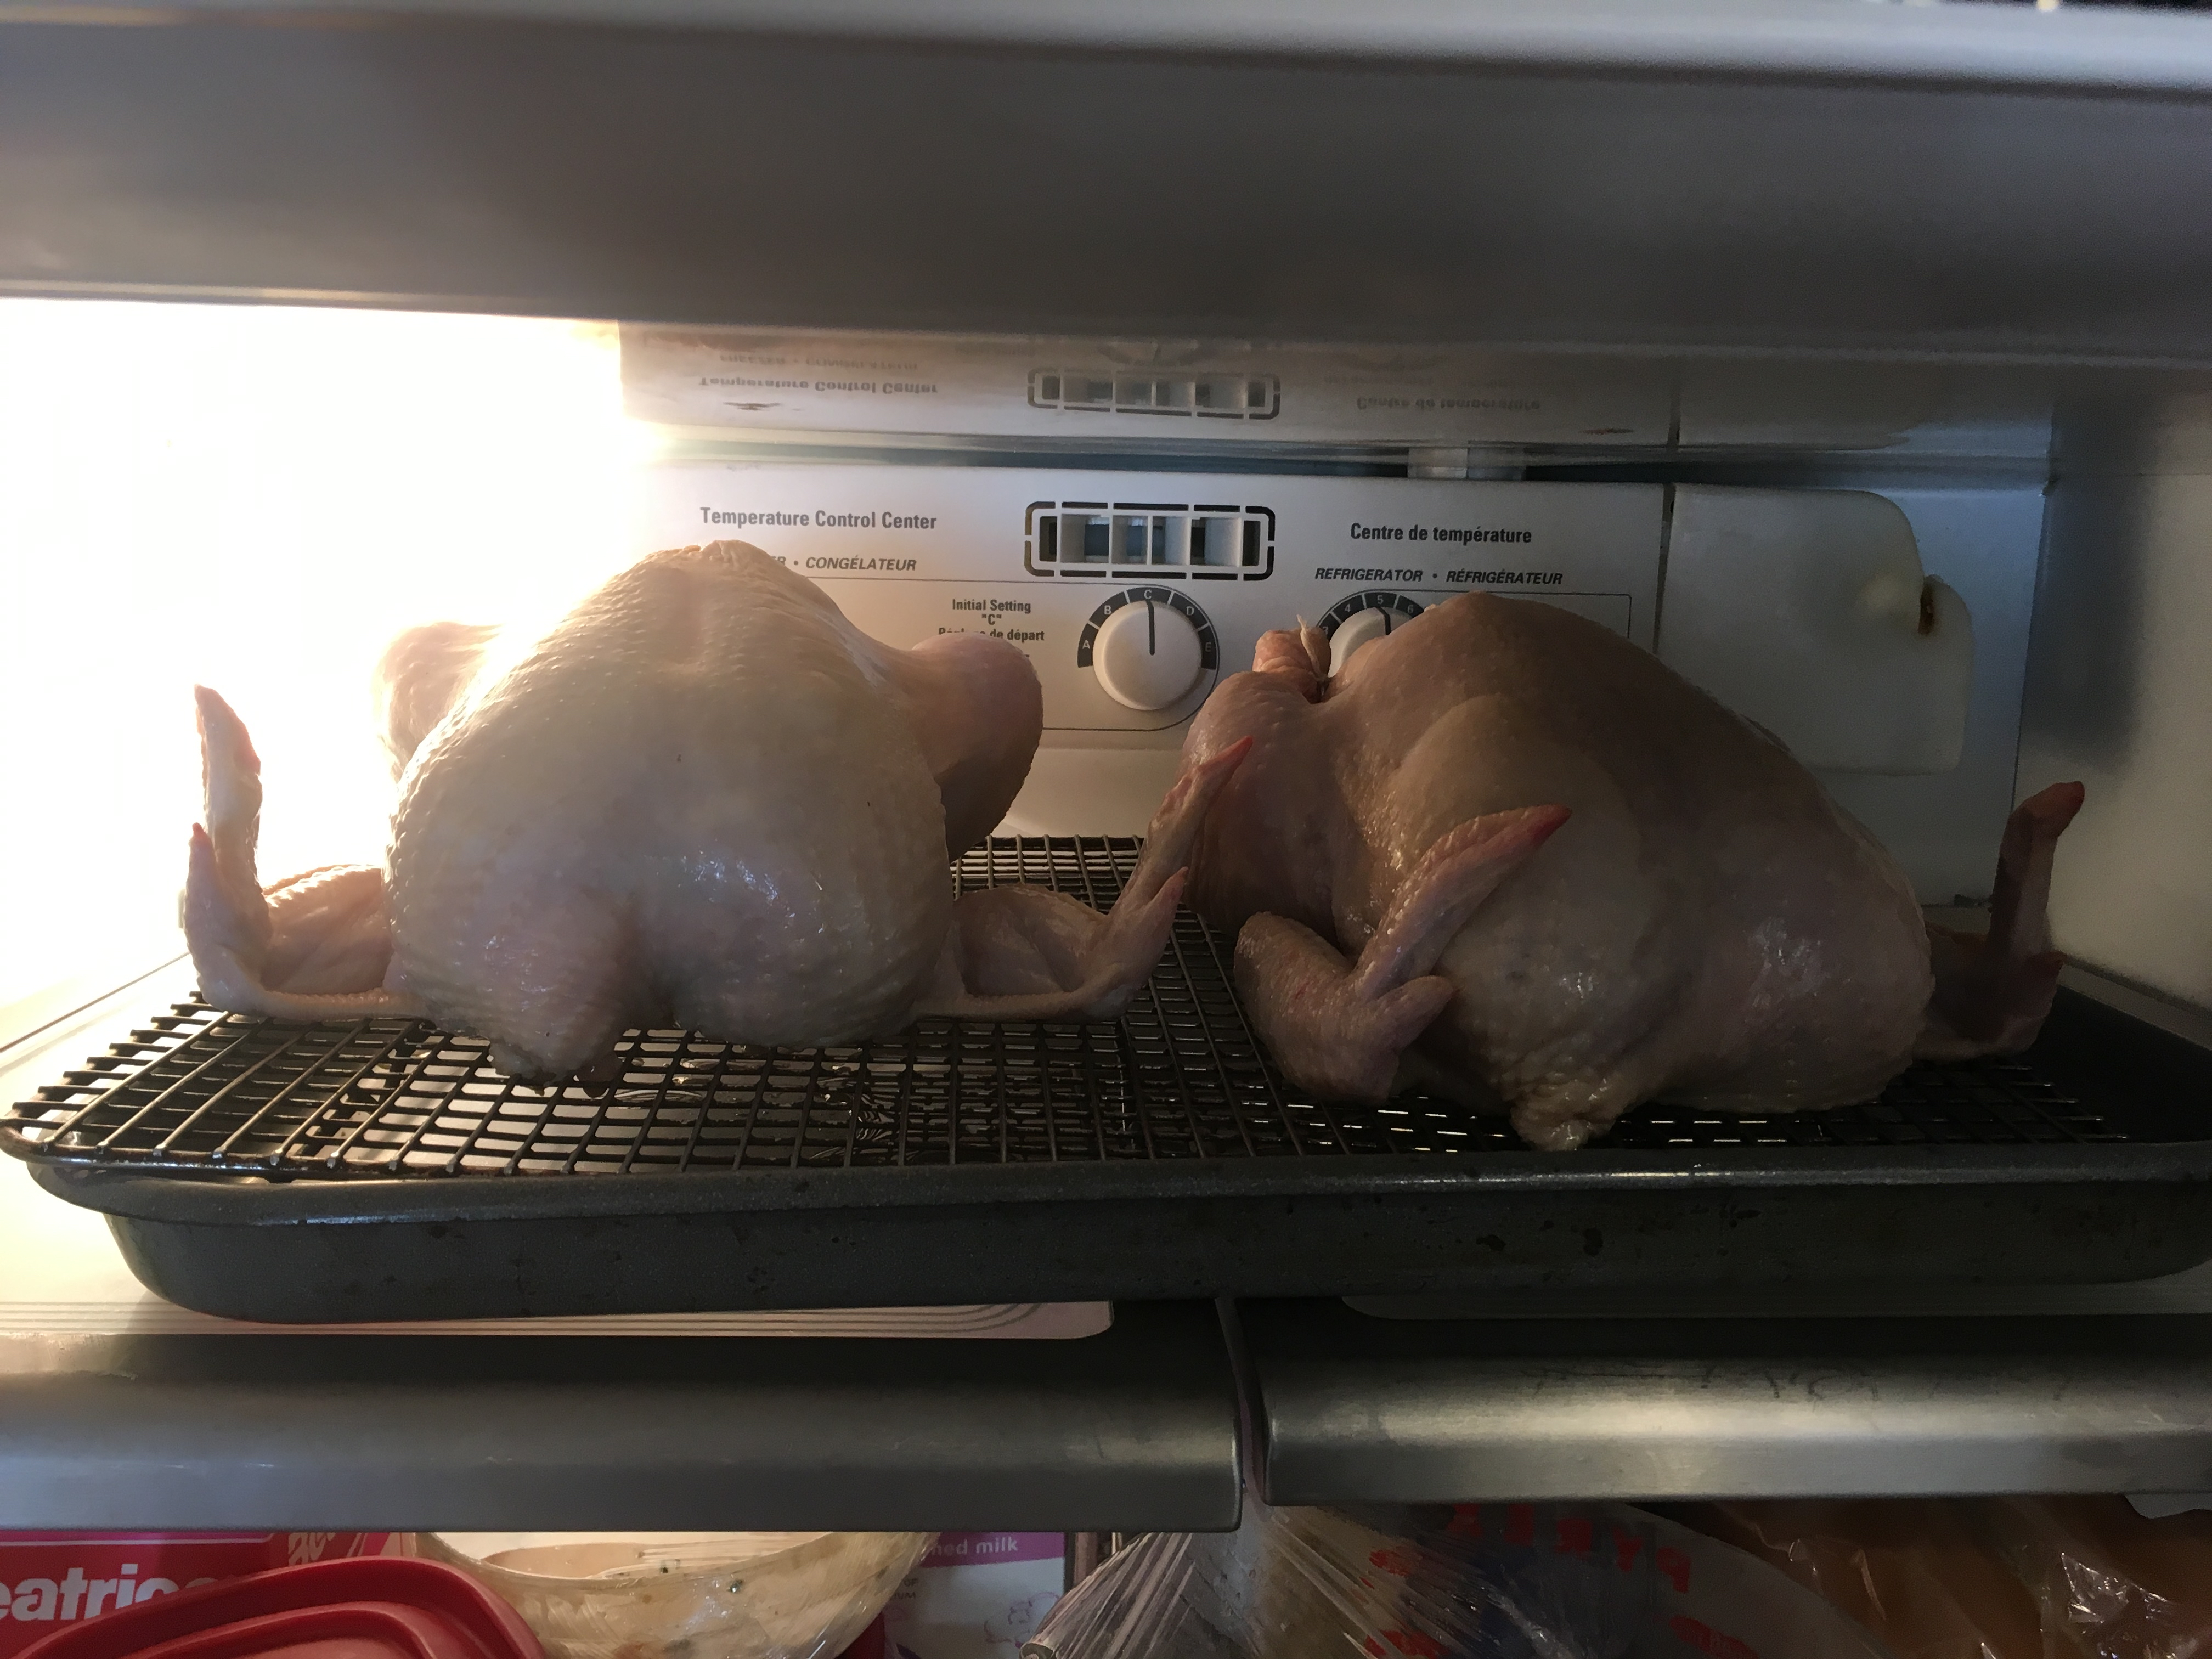
\includegraphics[width=0.25\textwidth]{\imageDir/\fileName/IMG_3220.jpg} &
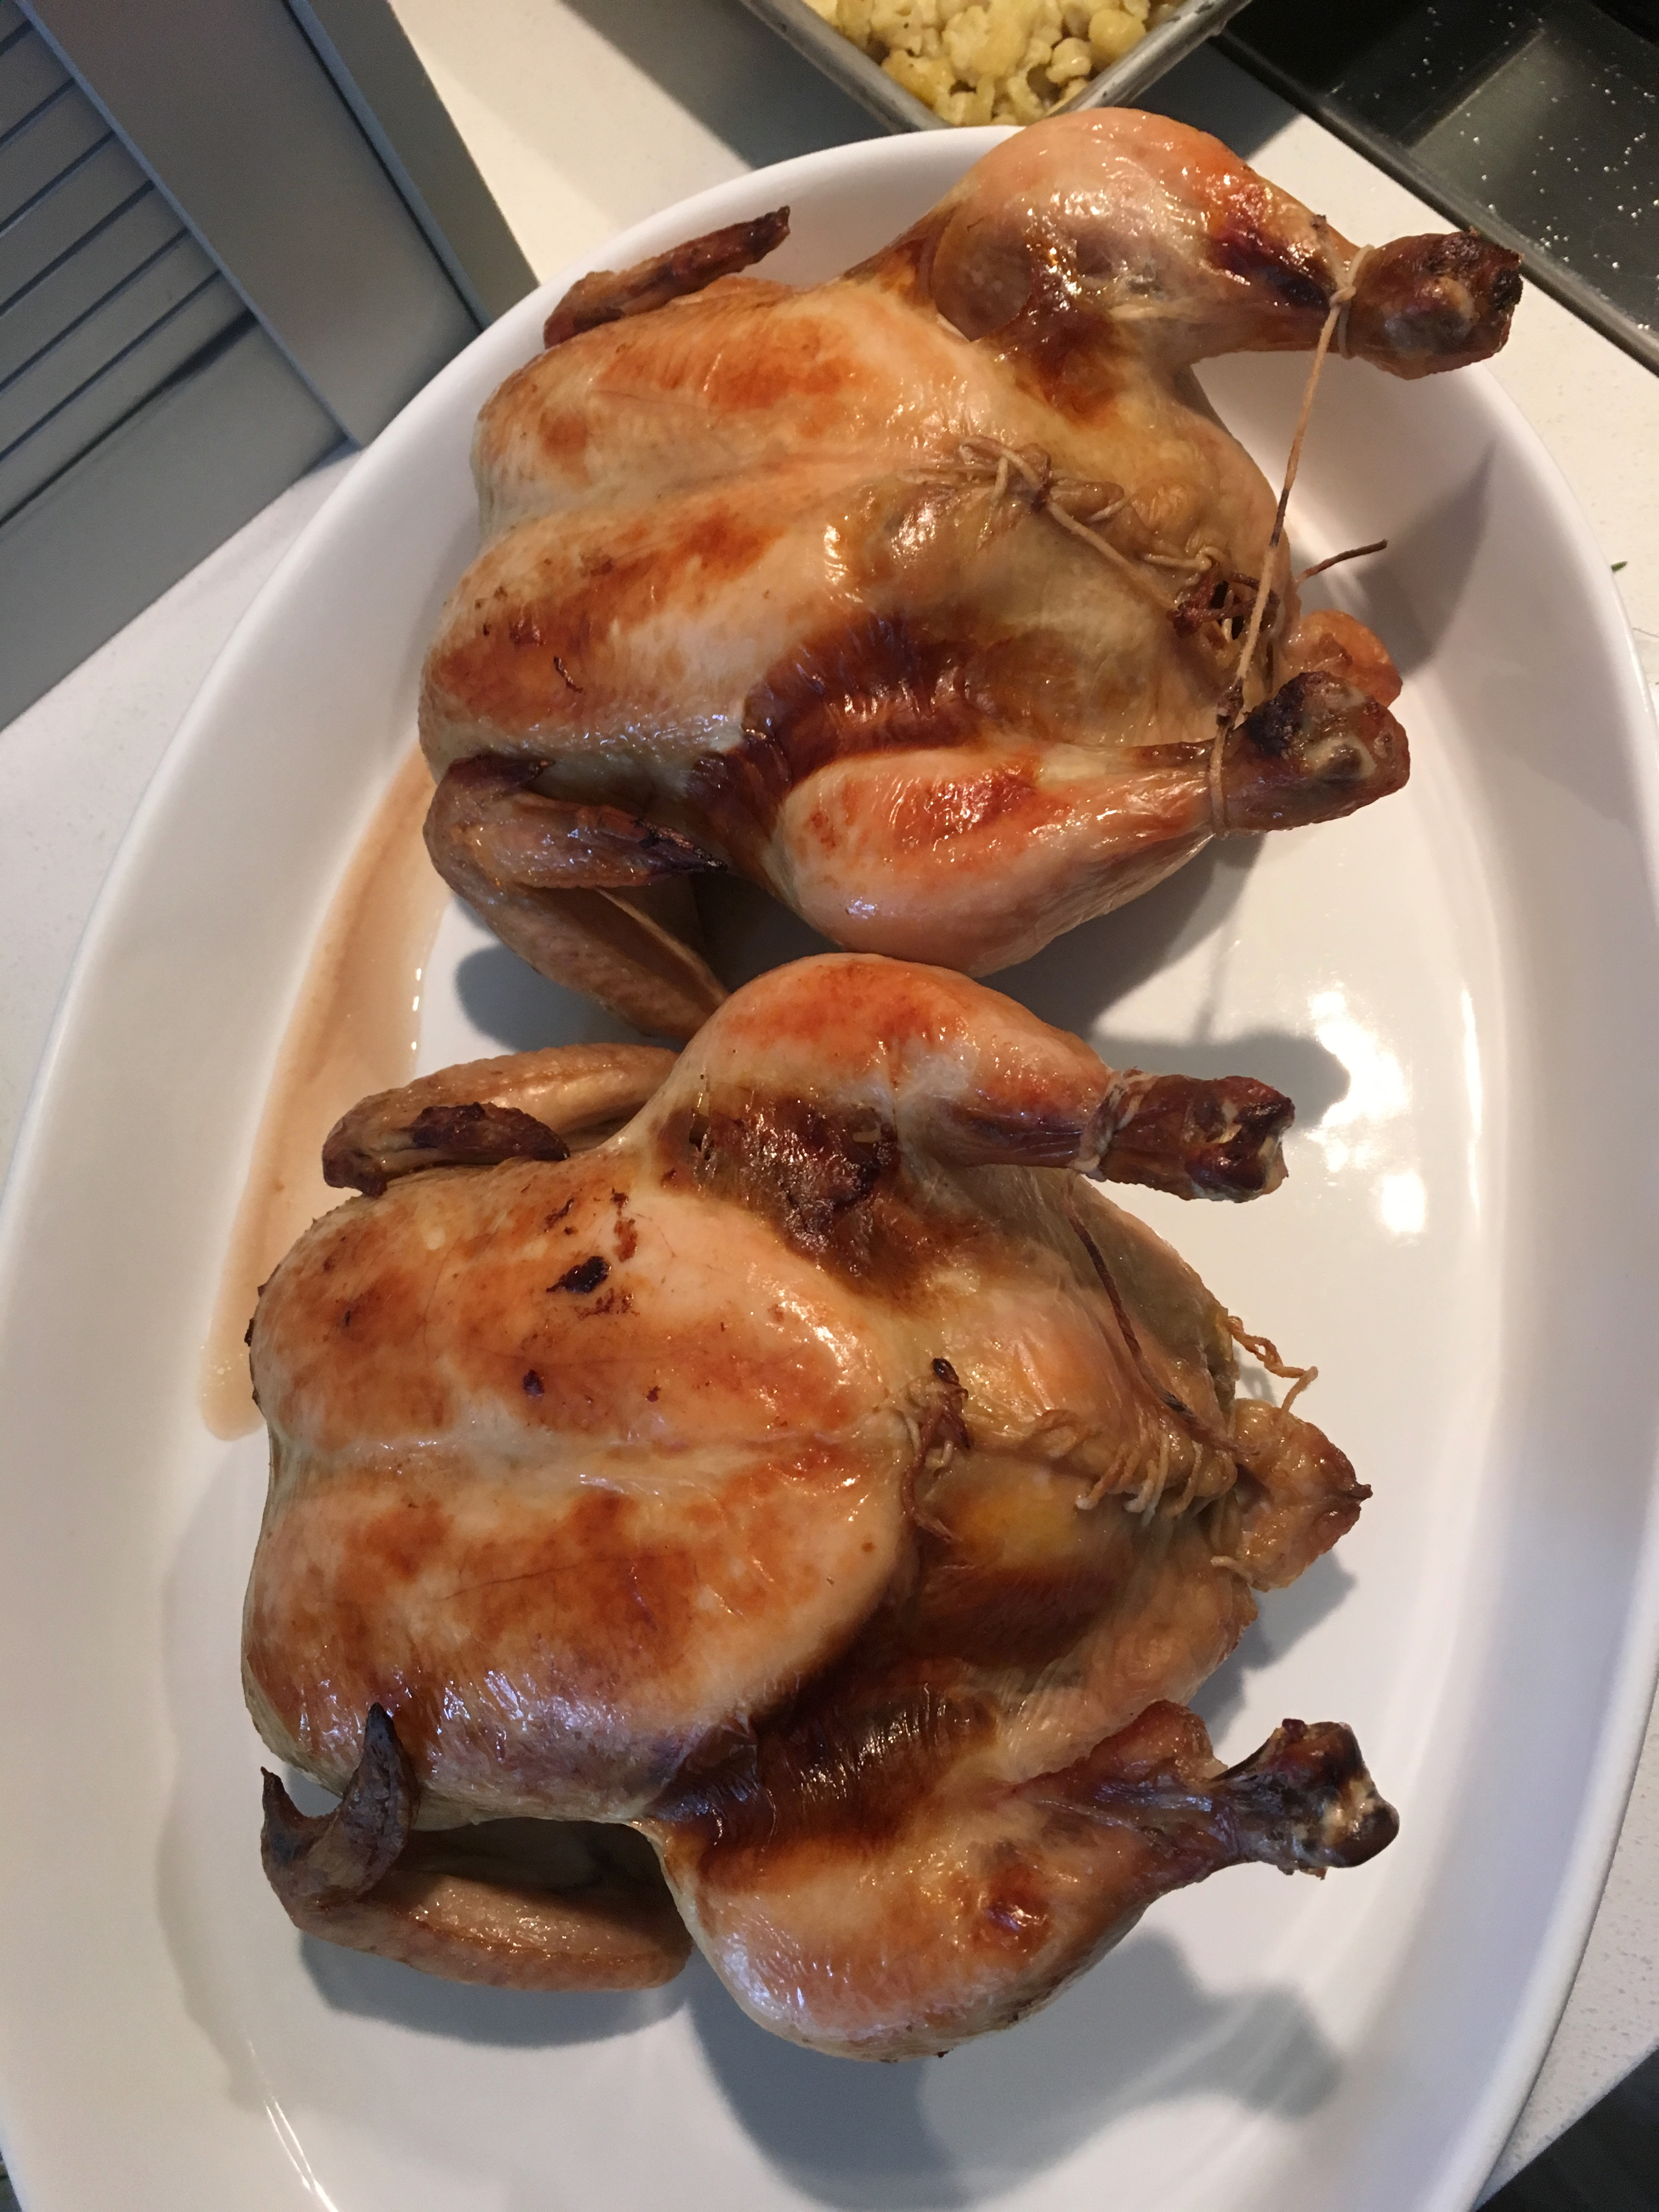
\includegraphics[width=0.25\textwidth]{\imageDir/\fileName/IMG_3228.jpg} \\
\end{tabular}
\end{table}

\end{document}



